% Options for packages loaded elsewhere
\PassOptionsToPackage{unicode}{hyperref}
\PassOptionsToPackage{hyphens}{url}
%
\documentclass[
]{article}
\usepackage{amsmath,amssymb}
\usepackage{iftex}
\ifPDFTeX
  \usepackage[T1]{fontenc}
  \usepackage[utf8]{inputenc}
  \usepackage{textcomp} % provide euro and other symbols
\else % if luatex or xetex
  \usepackage{unicode-math} % this also loads fontspec
  \defaultfontfeatures{Scale=MatchLowercase}
  \defaultfontfeatures[\rmfamily]{Ligatures=TeX,Scale=1}
\fi
\usepackage{lmodern}
\ifPDFTeX\else
  % xetex/luatex font selection
\fi
% Use upquote if available, for straight quotes in verbatim environments
\IfFileExists{upquote.sty}{\usepackage{upquote}}{}
\IfFileExists{microtype.sty}{% use microtype if available
  \usepackage[]{microtype}
  \UseMicrotypeSet[protrusion]{basicmath} % disable protrusion for tt fonts
}{}
\makeatletter
\@ifundefined{KOMAClassName}{% if non-KOMA class
  \IfFileExists{parskip.sty}{%
    \usepackage{parskip}
  }{% else
    \setlength{\parindent}{0pt}
    \setlength{\parskip}{6pt plus 2pt minus 1pt}}
}{% if KOMA class
  \KOMAoptions{parskip=half}}
\makeatother
\usepackage{xcolor}
\usepackage[margin=1in]{geometry}
\usepackage{longtable,booktabs,array}
\usepackage{calc} % for calculating minipage widths
% Correct order of tables after \paragraph or \subparagraph
\usepackage{etoolbox}
\makeatletter
\patchcmd\longtable{\par}{\if@noskipsec\mbox{}\fi\par}{}{}
\makeatother
% Allow footnotes in longtable head/foot
\IfFileExists{footnotehyper.sty}{\usepackage{footnotehyper}}{\usepackage{footnote}}
\makesavenoteenv{longtable}
\usepackage{graphicx}
\makeatletter
\def\maxwidth{\ifdim\Gin@nat@width>\linewidth\linewidth\else\Gin@nat@width\fi}
\def\maxheight{\ifdim\Gin@nat@height>\textheight\textheight\else\Gin@nat@height\fi}
\makeatother
% Scale images if necessary, so that they will not overflow the page
% margins by default, and it is still possible to overwrite the defaults
% using explicit options in \includegraphics[width, height, ...]{}
\setkeys{Gin}{width=\maxwidth,height=\maxheight,keepaspectratio}
% Set default figure placement to htbp
\makeatletter
\def\fps@figure{htbp}
\makeatother
\setlength{\emergencystretch}{3em} % prevent overfull lines
\providecommand{\tightlist}{%
  \setlength{\itemsep}{0pt}\setlength{\parskip}{0pt}}
\setcounter{secnumdepth}{5}
\usepackage{booktabs}
\usepackage{longtable}
\usepackage{array}
\usepackage{multirow}
\usepackage{wrapfig}
\usepackage{float}
\usepackage{colortbl}
\usepackage{pdflscape}
\usepackage{tabu}
\usepackage{threeparttable}
\usepackage{threeparttablex}
\usepackage[normalem]{ulem}
\usepackage{makecell}
\usepackage{xcolor}
\ifLuaTeX
  \usepackage{selnolig}  % disable illegal ligatures
\fi
\usepackage{bookmark}
\IfFileExists{xurl.sty}{\usepackage{xurl}}{} % add URL line breaks if available
\urlstyle{same}
\hypersetup{
  pdftitle={Through the eyes of the teacher - Multimodal exploration of expertise differences in the perception of classroom disruptions in a laboratory study},
  hidelinks,
  pdfcreator={LaTeX via pandoc}}

\title{Through the eyes of the teacher - Multimodal exploration of
expertise differences in the perception of classroom disruptions in a
laboratory study}
\author{}
\date{\vspace{-2.5em}}

\begin{document}
\maketitle

{
\setcounter{tocdepth}{2}
\tableofcontents
}
\subsection{1. Participants}\label{participants}

\begin{longtable}[]{@{}
  >{\raggedright\arraybackslash}p{(\columnwidth - 20\tabcolsep) * \real{0.0560}}
  >{\raggedleft\arraybackslash}p{(\columnwidth - 20\tabcolsep) * \real{0.0240}}
  >{\raggedleft\arraybackslash}p{(\columnwidth - 20\tabcolsep) * \real{0.1360}}
  >{\raggedleft\arraybackslash}p{(\columnwidth - 20\tabcolsep) * \real{0.1200}}
  >{\raggedleft\arraybackslash}p{(\columnwidth - 20\tabcolsep) * \real{0.1280}}
  >{\raggedleft\arraybackslash}p{(\columnwidth - 20\tabcolsep) * \real{0.1360}}
  >{\raggedleft\arraybackslash}p{(\columnwidth - 20\tabcolsep) * \real{0.1360}}
  >{\raggedleft\arraybackslash}p{(\columnwidth - 20\tabcolsep) * \real{0.0560}}
  >{\raggedleft\arraybackslash}p{(\columnwidth - 20\tabcolsep) * \real{0.0640}}
  >{\raggedleft\arraybackslash}p{(\columnwidth - 20\tabcolsep) * \real{0.0720}}
  >{\raggedleft\arraybackslash}p{(\columnwidth - 20\tabcolsep) * \real{0.0720}}@{}}
\caption{Demographic information \& teaching experience}\tabularnewline
\toprule\noalign{}
\begin{minipage}[b]{\linewidth}\raggedright
Group
\end{minipage} & \begin{minipage}[b]{\linewidth}\raggedleft
N
\end{minipage} & \begin{minipage}[b]{\linewidth}\raggedleft
Women in percent
\end{minipage} & \begin{minipage}[b]{\linewidth}\raggedleft
M Age in years
\end{minipage} & \begin{minipage}[b]{\linewidth}\raggedleft
SD Age in years
\end{minipage} & \begin{minipage}[b]{\linewidth}\raggedleft
Min Age in years
\end{minipage} & \begin{minipage}[b]{\linewidth}\raggedleft
Max Age in years
\end{minipage} & \begin{minipage}[b]{\linewidth}\raggedleft
M Exp.
\end{minipage} & \begin{minipage}[b]{\linewidth}\raggedleft
SD Exp.
\end{minipage} & \begin{minipage}[b]{\linewidth}\raggedleft
Min Exp.
\end{minipage} & \begin{minipage}[b]{\linewidth}\raggedleft
Max Exp.
\end{minipage} \\
\midrule\noalign{}
\endfirsthead
\toprule\noalign{}
\begin{minipage}[b]{\linewidth}\raggedright
Group
\end{minipage} & \begin{minipage}[b]{\linewidth}\raggedleft
N
\end{minipage} & \begin{minipage}[b]{\linewidth}\raggedleft
Women in percent
\end{minipage} & \begin{minipage}[b]{\linewidth}\raggedleft
M Age in years
\end{minipage} & \begin{minipage}[b]{\linewidth}\raggedleft
SD Age in years
\end{minipage} & \begin{minipage}[b]{\linewidth}\raggedleft
Min Age in years
\end{minipage} & \begin{minipage}[b]{\linewidth}\raggedleft
Max Age in years
\end{minipage} & \begin{minipage}[b]{\linewidth}\raggedleft
M Exp.
\end{minipage} & \begin{minipage}[b]{\linewidth}\raggedleft
SD Exp.
\end{minipage} & \begin{minipage}[b]{\linewidth}\raggedleft
Min Exp.
\end{minipage} & \begin{minipage}[b]{\linewidth}\raggedleft
Max Exp.
\end{minipage} \\
\midrule\noalign{}
\endhead
\bottomrule\noalign{}
\endlastfoot
Expert & 40 & 60.00 & 39.10 & 10.55 & 26 & 60 & 11.55 & 11.32 & 1 &
38 \\
Novice & 42 & 69.05 & 22.83 & 1.85 & 19 & 27 & 0.00 & 0.00 & 0 & 0 \\
\end{longtable}

\subsection{2. Measures}\label{measures}

\subsubsection{2.1 Eye-Tracking Data}\label{eye-tracking-data}

\paragraph{2.2.2 Letter search}\label{letter-search}

\begin{longtable}[]{@{}lrrrrr@{}}
\caption{N, M, SD, min \& max letter search in seconds}\tabularnewline
\toprule\noalign{}
Group & N & M & SD & Min & Max \\
\midrule\noalign{}
\endfirsthead
\toprule\noalign{}
Group & N & M & SD & Min & Max \\
\midrule\noalign{}
\endhead
\bottomrule\noalign{}
\endlastfoot
Expert & 39 & 12.97 & 6.75 & 2.72 & 29.24 \\
Novice & 40 & 12.22 & 8.79 & 2.28 & 48.26 \\
\end{longtable}

\paragraph{t-test \& effect size ``Letter
search''}\label{t-test-effect-size-letter-search}

\begin{verbatim}
Two Sample t-test
\end{verbatim}

data: df\_letter\(Duration_of_interval_sec[df_letter\)Group ==
``Expert''{]} and df\_letter\(Duration_of_interval_sec[df_letter\)Group
== ``Novice''{]} t = 0.42858, df = 77, p-value = 0.6694 alternative
hypothesis: true difference in means is not equal to 0 95 percent
confidence interval: -2.760420 4.274574 sample estimates: mean of x mean
of y 12.97308 12.21600

{[}1{]} 0.1 attr(,``magnitude'') {[}1{]} ``negligible''

\paragraph{2.2.1 Number of fixations per minute (micro-teaching
unit)}\label{number-of-fixations-per-minute-micro-teaching-unit}

\begin{longtable}[]{@{}lrrrrr@{}}
\caption{N, M, SD, min \& max number of fixation per minute
(micro-teaching unit)}\tabularnewline
\toprule\noalign{}
Group & N & M & SD & Min & Max \\
\midrule\noalign{}
\endfirsthead
\toprule\noalign{}
Group & N & M & SD & Min & Max \\
\midrule\noalign{}
\endhead
\bottomrule\noalign{}
\endlastfoot
Novice & 42 & 91.26 & 14.43 & 69 & 123 \\
Expert & 40 & 98.58 & 19.04 & 49 & 136 \\
\end{longtable}

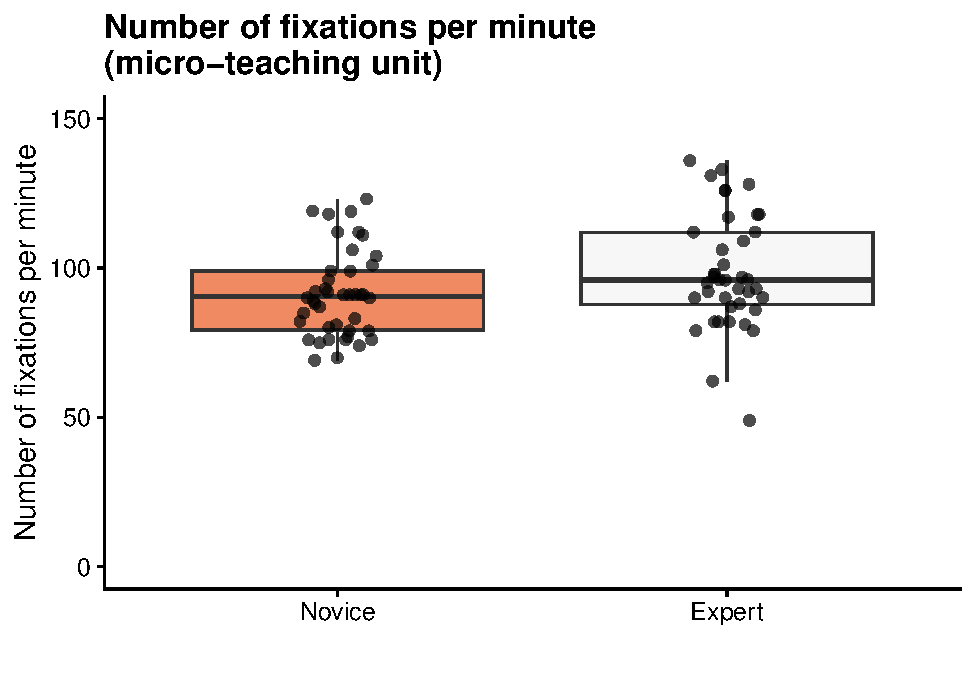
\includegraphics{expertise_2024_09_26_no_outlierdetection_MK_files/figure-latex/nof_all-1.pdf}

\paragraph{t-test \& effect size ``Number of fixation (micro-teaching
unit)''}\label{t-test-effect-size-number-of-fixation-micro-teaching-unit}

\begin{verbatim}
Two Sample t-test
\end{verbatim}

data: df\_aoi\_sum\(Number_fixation_min_mtu[df_aoi_sum\)Group ==
``Expert''{]} and
df\_aoi\_sum\(Number_fixation_min_mtu[df_aoi_sum\)Group == ``Novice''{]}
t = 1.966, df = 80, p-value = 0.05276 alternative hypothesis: true
difference in means is not equal to 0 95 percent confidence interval:
-0.08935625 14.71554673 sample estimates: mean of x mean of y 98.5750
91.2619

{[}1{]} 0.43 attr(,``magnitude'') {[}1{]} ``small''

\paragraph{2.2.2 Number of fixations per minute (AOI
students)}\label{number-of-fixations-per-minute-aoi-students}

\begin{longtable}[]{@{}lrrrrr@{}}
\caption{N, M, SD, min \& max number of fixations per minute (AOI
students)}\tabularnewline
\toprule\noalign{}
Group & N & M & SD & Min & Max \\
\midrule\noalign{}
\endfirsthead
\toprule\noalign{}
Group & N & M & SD & Min & Max \\
\midrule\noalign{}
\endhead
\bottomrule\noalign{}
\endlastfoot
Novice & 42 & 40.08 & 11.58 & 16.91 & 61.53 \\
Expert & 40 & 43.26 & 12.55 & 25.06 & 74.31 \\
\end{longtable}

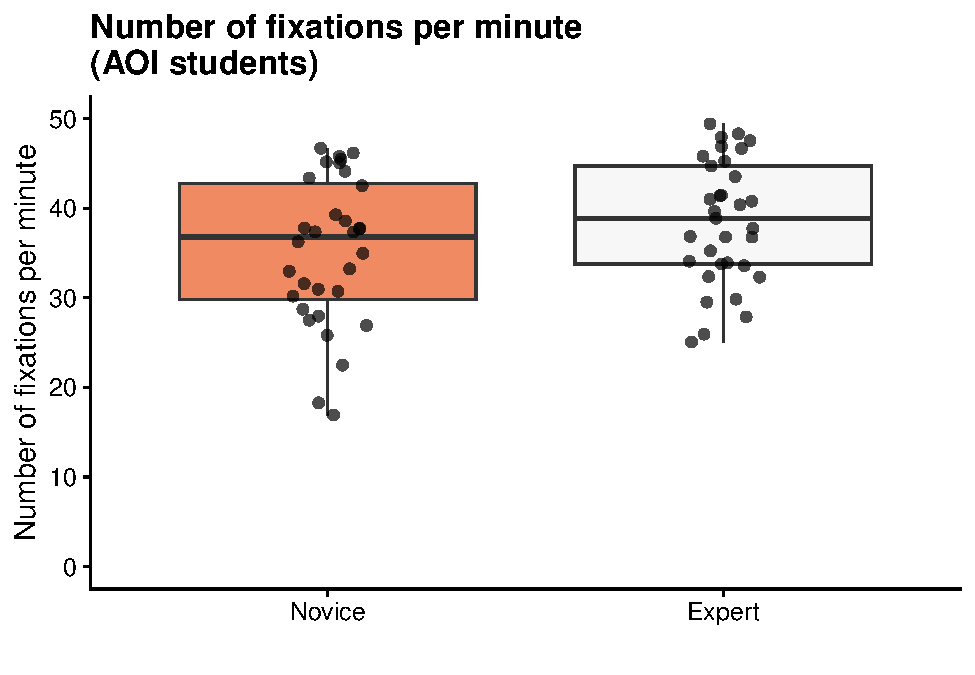
\includegraphics{expertise_2024_09_26_no_outlierdetection_MK_files/figure-latex/nof_students-1.pdf}

\paragraph{t-test \& effect size ``Number of fixation'' (AOI
students)}\label{t-test-effect-size-number-of-fixation-aoi-students}

\begin{verbatim}
Two Sample t-test
\end{verbatim}

data: df\_aoi\_stud\(Stud_number_fixation_min[df_aoi_stud\)Group ==
``Expert''{]} and
df\_aoi\_stud\(Stud_number_fixation_min[df_aoi_stud\)Group ==
``Novice''{]} t = 1.1925, df = 80, p-value = 0.2366 alternative
hypothesis: true difference in means is not equal to 0 95 percent
confidence interval: -2.125346 8.480489 sample estimates: mean of x mean
of y 43.25900 40.08143

{[}1{]} 0.26 attr(,``magnitude'') {[}1{]} ``small''

\paragraph{2.2.3 Number of fixations (AOI disruptive
person)}\label{number-of-fixations-aoi-disruptive-person}

\begin{longtable}[]{@{}lrrrrr@{}}
\caption{N, M, SD, min \& max number of fixation (AOI disruptive
person)}\tabularnewline
\toprule\noalign{}
Group & N & M & SD & Min & Max \\
\midrule\noalign{}
\endfirsthead
\toprule\noalign{}
Group & N & M & SD & Min & Max \\
\midrule\noalign{}
\endhead
\bottomrule\noalign{}
\endlastfoot
Novice & 42 & 48.14 & 21.87 & 25 & 133 \\
Expert & 40 & 44.12 & 13.31 & 15 & 88 \\
\end{longtable}

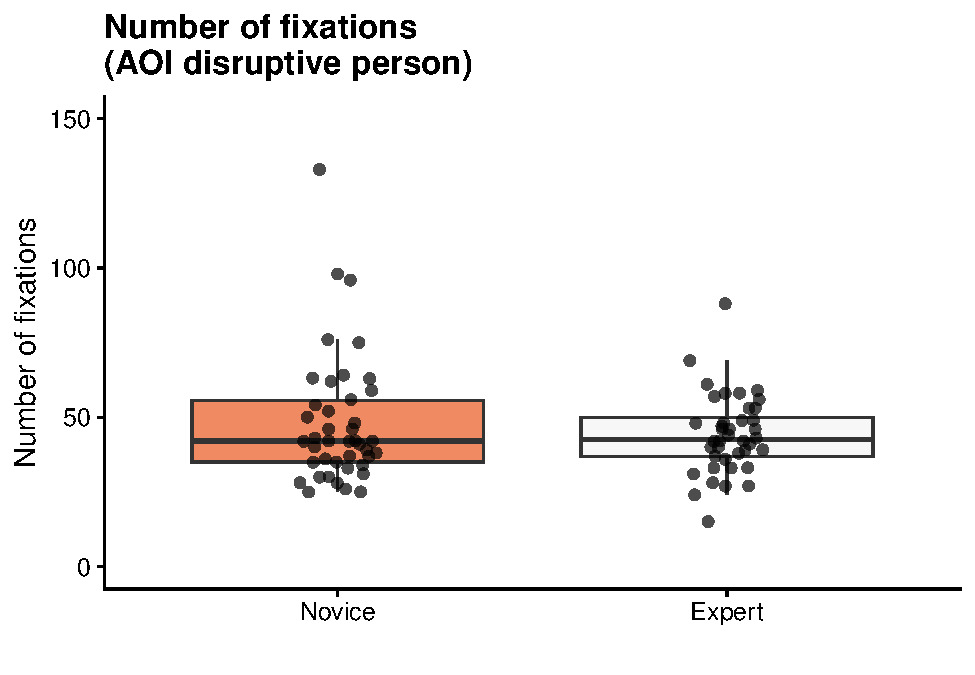
\includegraphics{expertise_2024_09_26_no_outlierdetection_MK_files/figure-latex/nof_disrup-1.pdf}

\paragraph{t-test \& effect size ``Number of fixations'' (AOI disruptive
person)}\label{t-test-effect-size-number-of-fixations-aoi-disruptive-person}

\begin{verbatim}
Two Sample t-test
\end{verbatim}

data:
df\_aoi\_disrup\(Number_of_fixations.Disruptive_Person[df_aoi_disrup\)Group
== ``Expert''{]} and
df\_aoi\_disrup\(Number_of_fixations.Disruptive_Person[df_aoi_disrup\)Group
== ``Novice''{]} t = -0.99886, df = 80, p-value = 0.3209 alternative
hypothesis: true difference in means is not equal to 0 95 percent
confidence interval: -12.022778 3.987063 sample estimates: mean of x
mean of y 44.12500 48.14286

{[}1{]} -0.22 attr(,``magnitude'') {[}1{]} ``small''

\paragraph{2.2.4 Average duration of fixations in milliseconds
(micro-teaching
unit)}\label{average-duration-of-fixations-in-milliseconds-micro-teaching-unit}

\begin{longtable}[]{@{}lrrrrr@{}}
\caption{N, M, SD, min \& max duration of fixations in milliseconds
(micro-teaching unit)}\tabularnewline
\toprule\noalign{}
Group & N & M in ms & SD in ms & Min in ms & Max in ms \\
\midrule\noalign{}
\endfirsthead
\toprule\noalign{}
Group & N & M in ms & SD in ms & Min in ms & Max in ms \\
\midrule\noalign{}
\endhead
\bottomrule\noalign{}
\endlastfoot
Novice & 42 & 513.81 & 117.71 & 247 & 749 \\
Expert & 40 & 472.92 & 106.18 & 295 & 712 \\
\end{longtable}

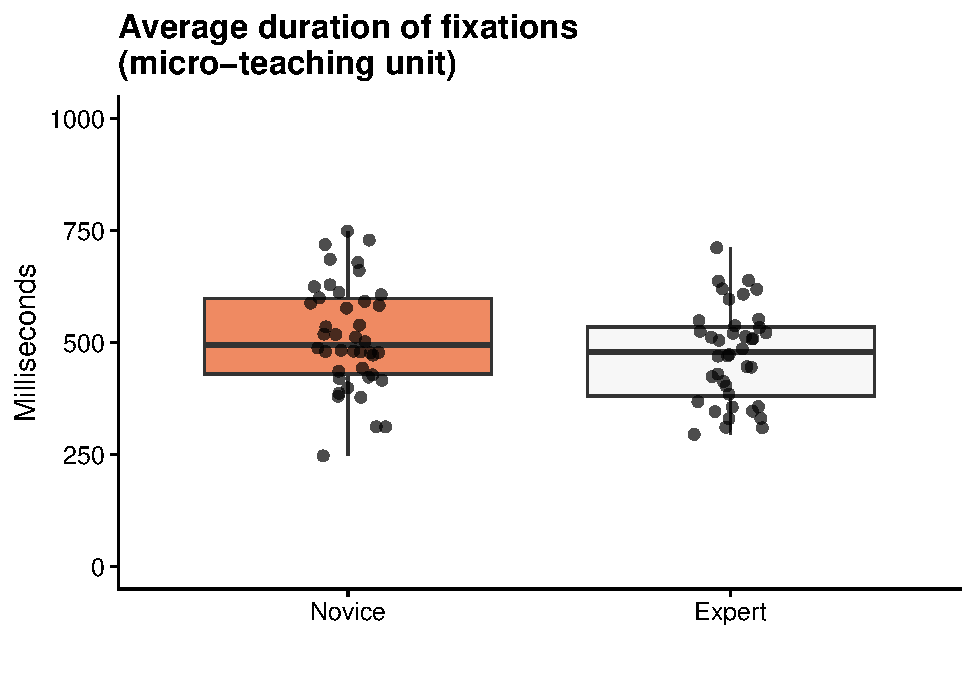
\includegraphics{expertise_2024_09_26_no_outlierdetection_MK_files/figure-latex/dur_all-1.pdf}

\paragraph{t-test \& effect size ``Average duration of fixations''
(micro-teaching
unit)}\label{t-test-effect-size-average-duration-of-fixations-micro-teaching-unit}

\begin{verbatim}
Two Sample t-test
\end{verbatim}

data: df\_aoi\_sum\(Average_duration_mtu[df_aoi_sum\)Group ==
``Expert''{]} and df\_aoi\_sum\(Average_duration_mtu[df_aoi_sum\)Group
== ``Novice''{]} t = -1.6488, df = 80, p-value = 0.1031 alternative
hypothesis: true difference in means is not equal to 0 95 percent
confidence interval: -90.231822 8.462774 sample estimates: mean of x
mean of y 472.9250 513.8095

{[}1{]} -0.36 attr(,``magnitude'') {[}1{]} ``small''

\paragraph{2.2.5 Average duration of fixations (AOI
students)}\label{average-duration-of-fixations-aoi-students}

\begin{longtable}[]{@{}lrrrrr@{}}
\caption{N, M, SD, min \& max average duration of fixations in
milliseconds (AOI students)}\tabularnewline
\toprule\noalign{}
Group & N & M in ms & SD in ms & Min in ms & Max in ms \\
\midrule\noalign{}
\endfirsthead
\toprule\noalign{}
Group & N & M in ms & SD in ms & Min in ms & Max in ms \\
\midrule\noalign{}
\endhead
\bottomrule\noalign{}
\endlastfoot
Novice & 42 & 613.67 & 191.19 & 254 & 1115 \\
Expert & 40 & 552.55 & 146.32 & 309 & 925 \\
\end{longtable}

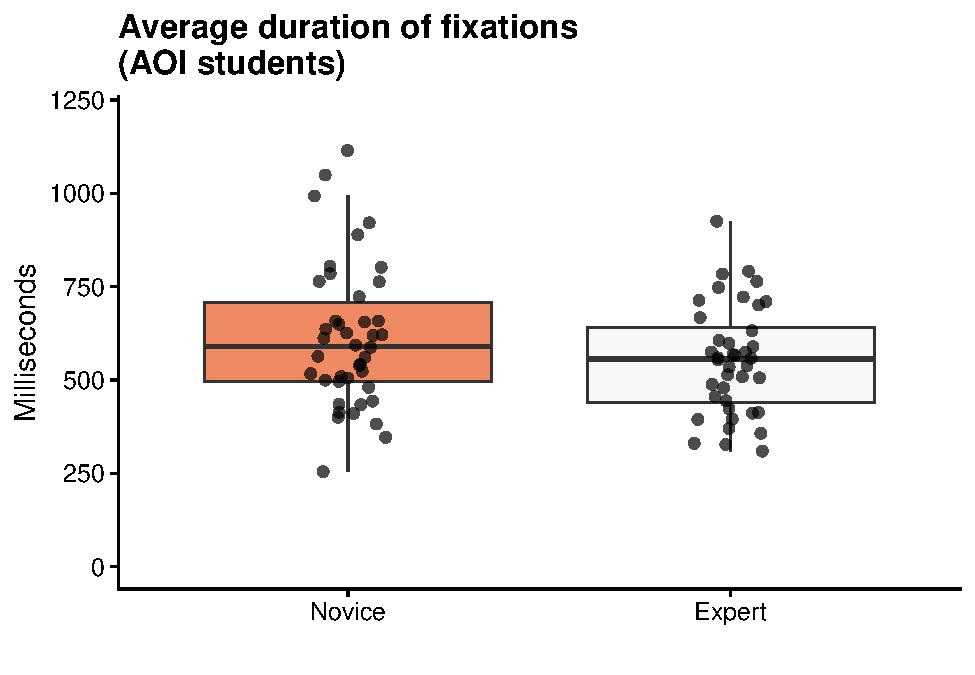
\includegraphics{expertise_2024_09_26_no_outlierdetection_MK_files/figure-latex/dur_students-1.pdf}

\paragraph{t-test \& effect size ``Average duration of fixations'' (AOI
students)}\label{t-test-effect-size-average-duration-of-fixations-aoi-students}

\begin{verbatim}
Two Sample t-test
\end{verbatim}

data: df\_aoi\_stud\(Average_duration_stud[df_aoi_stud\)Group ==
``Expert''{]} and
df\_aoi\_stud\(Average_duration_stud[df_aoi_stud\)Group == ``Novice''{]}
t = -1.6197, df = 80, p-value = 0.1092 alternative hypothesis: true
difference in means is not equal to 0 95 percent confidence interval:
-136.20902 13.97569 sample estimates: mean of x mean of y 552.5500
613.6667

{[}1{]} -0.36 attr(,``magnitude'') {[}1{]} ``small''

\paragraph{2.2.6 Average duration of fixations (AOI disruptive
person)}\label{average-duration-of-fixations-aoi-disruptive-person}

\begin{longtable}[]{@{}lrrrrr@{}}
\caption{N, M, SD, min \& max average duration of fixations in
milliseconds (AOI disruptive person)}\tabularnewline
\toprule\noalign{}
Group & N & M in ms & SD in ms & Min in ms & Max in ms \\
\midrule\noalign{}
\endfirsthead
\toprule\noalign{}
Group & N & M in ms & SD in ms & Min in ms & Max in ms \\
\midrule\noalign{}
\endhead
\bottomrule\noalign{}
\endlastfoot
Novice & 42 & 584.57 & 216.40 & 266 & 1150 \\
Expert & 40 & 503.05 & 153.92 & 303 & 1081 \\
\end{longtable}

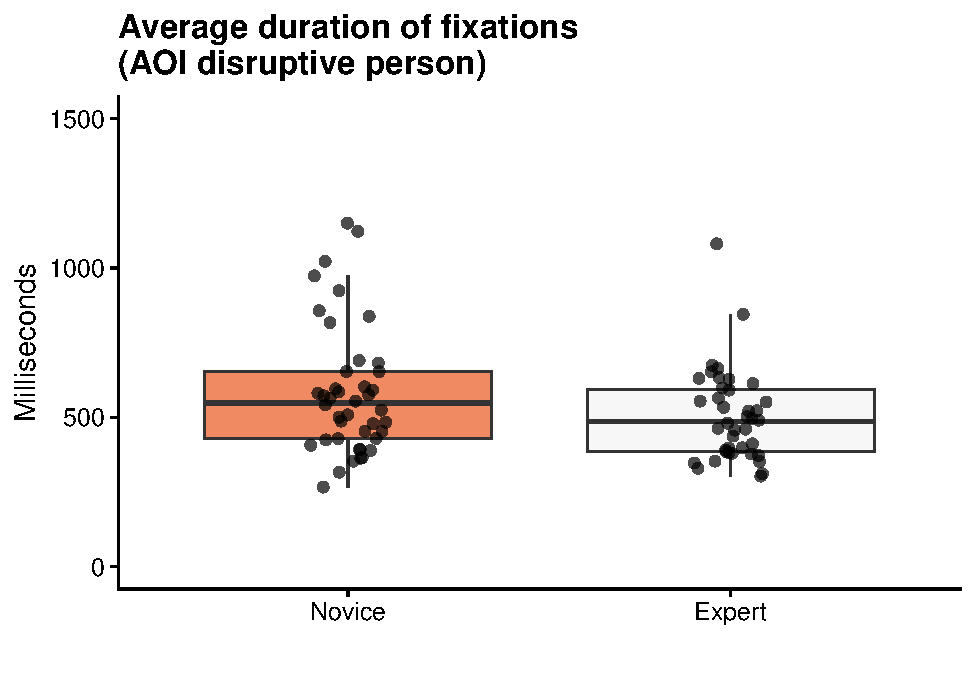
\includegraphics{expertise_2024_09_26_no_outlierdetection_MK_files/figure-latex/dur_disrup-1.pdf}

\paragraph{t-test \& effect size ``Average duration of fixations'' (AOI
disruptive
person)}\label{t-test-effect-size-average-duration-of-fixations-aoi-disruptive-person}

\begin{verbatim}
Two Sample t-test
\end{verbatim}

data: df\_aoi\_disrup\(Average_duration_disrup[df_aoi_disrup\)Group ==
``Expert''{]} and
df\_aoi\_disrup\(Average_duration_disrup[df_aoi_disrup\)Group ==
``Novice''{]} t = -1.957, df = 80, p-value = 0.05383 alternative
hypothesis: true difference in means is not equal to 0 95 percent
confidence interval: -164.418963 1.376106 sample estimates: mean of x
mean of y 503.0500 584.5714

{[}1{]} -0.43 attr(,``magnitude'') {[}1{]} ``small''

\paragraph{2.2.7 Gaze Relational Index (GRI; micro-teaching
unit)}\label{gaze-relational-index-gri-micro-teaching-unit}

\begin{longtable}[]{@{}lrrrrr@{}}
\caption{N, M, SD, min \& max GRI (micro-teaching unit)}\tabularnewline
\toprule\noalign{}
Group & N & M & SD & Min & Max \\
\midrule\noalign{}
\endfirsthead
\toprule\noalign{}
Group & N & M & SD & Min & Max \\
\midrule\noalign{}
\endhead
\bottomrule\noalign{}
\endlastfoot
Novice & 42 & 5.93 & 2.11 & 2.08 & 10.70 \\
Expert & 40 & 5.18 & 2.13 & 2.17 & 11.48 \\
\end{longtable}

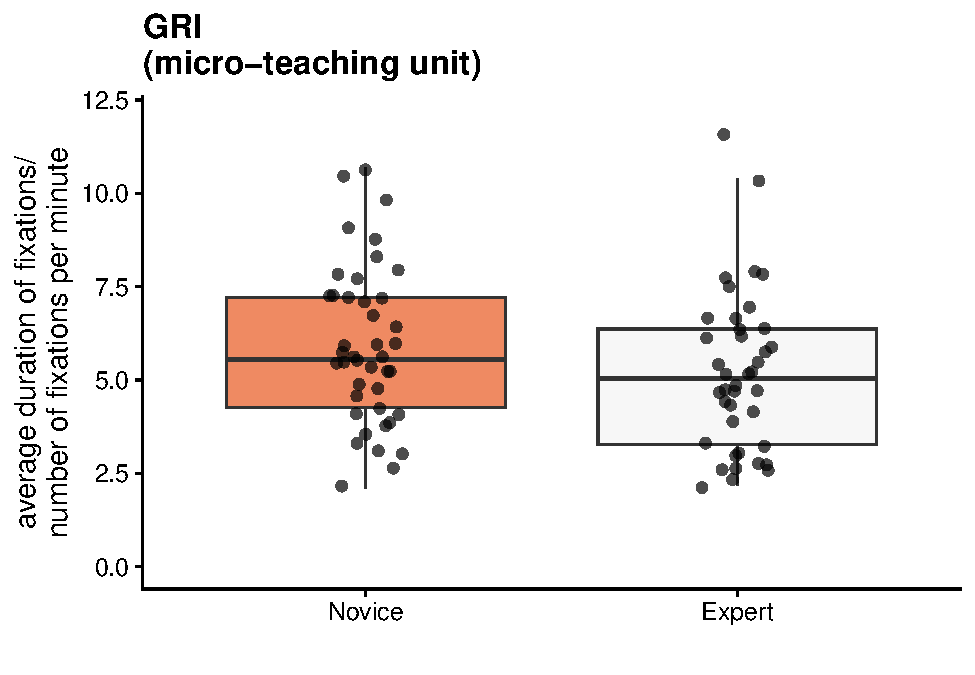
\includegraphics{expertise_2024_09_26_no_outlierdetection_MK_files/figure-latex/gri_all-1.pdf}

\paragraph{t-test \& effect size ``GRI'' (micro-teaching
unit)}\label{t-test-effect-size-gri-micro-teaching-unit}

\begin{verbatim}
Two Sample t-test
\end{verbatim}

data: df\_gri\(GRI[df_gri\)Group == ``Expert''{]} and
df\_gri\(GRI[df_gri\)Group == ``Novice''{]} t = -1.5975, df = 80,
p-value = 0.1141 alternative hypothesis: true difference in means is not
equal to 0 95 percent confidence interval: -1.682021 0.184045 sample
estimates: mean of x mean of y 5.176250 5.925238

{[}1{]} -0.35 attr(,``magnitude'') {[}1{]} ``small''

\paragraph{2.2.10 Time to first fixation in seconds (AOI disruptive
person)}\label{time-to-first-fixation-in-seconds-aoi-disruptive-person}

\begin{longtable}[]{@{}lrrrrr@{}}
\caption{N, M, SD, min \& max time to first fixation in seconds (AOI
disruptive person)}\tabularnewline
\toprule\noalign{}
Group & N & M in sec & SD in sec & Min in sec & Max in sec \\
\midrule\noalign{}
\endfirsthead
\toprule\noalign{}
Group & N & M in sec & SD in sec & Min in sec & Max in sec \\
\midrule\noalign{}
\endhead
\bottomrule\noalign{}
\endlastfoot
Expert & 39 & 3.57 & 2.18 & 0.25 & 8.78 \\
Novice & 40 & 3.79 & 1.80 & 0.72 & 8.89 \\
\end{longtable}

\begin{longtable}[]{@{}lrrrr@{}}
\caption{N, M, SD, min \& max of the perceived ´disruptive
person´}\tabularnewline
\toprule\noalign{}
Group & Mean & SD & Min & Max \\
\midrule\noalign{}
\endfirsthead
\toprule\noalign{}
Group & Mean & SD & Min & Max \\
\midrule\noalign{}
\endhead
\bottomrule\noalign{}
\endlastfoot
Expert & 6.82 & 1.60 & 4 & 9 \\
Novice & 6.90 & 1.43 & 3 & 9 \\
\end{longtable}

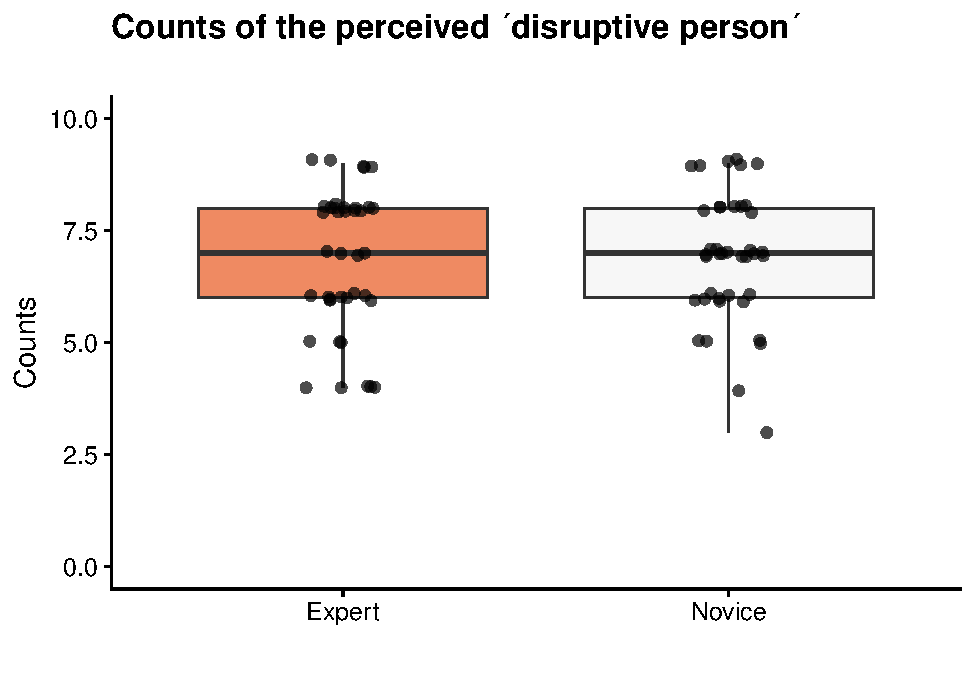
\includegraphics{expertise_2024_09_26_no_outlierdetection_MK_files/figure-latex/ttff_disrup-1.pdf}
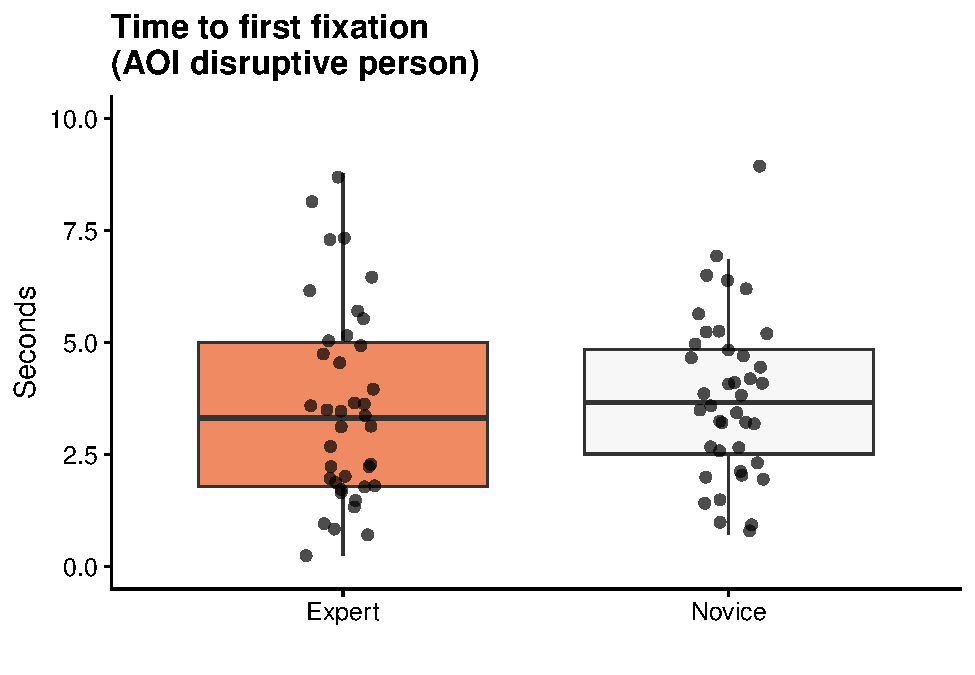
\includegraphics{expertise_2024_09_26_no_outlierdetection_MK_files/figure-latex/ttff_disrup-2.pdf}

\paragraph{t-test \& effect size ``Time to first fixation'' (AOI
disruptive
person)}\label{t-test-effect-size-time-to-first-fixation-aoi-disruptive-person}

\begin{verbatim}
Two Sample t-test
\end{verbatim}

data: df\_ttff\_disrup\(Disrup_time_fixation_sec[df_ttff_disrup\)Group
== ``Expert''{]} and
df\_ttff\_disrup\(Disrup_time_fixation_sec[df_ttff_disrup\)Group ==
``Novice''{]} t = -0.67144, df = 80, p-value = 0.5039 alternative
hypothesis: true difference in means is not equal to 0 95 percent
confidence interval: -1.4276630 0.7073296 sample estimates: mean of x
mean of y 3.766500 4.126667

{[}1{]} -0.15 attr(,``magnitude'') {[}1{]} ``negligible''

\subsubsection{2.2 Rating Scales (Disruption Appraisal, Confidence
Appraisal, Prevalence
Rating)}\label{rating-scales-disruption-appraisal-confidence-appraisal-prevalence-rating}

\begin{longtable}[]{@{}lrrrrr@{}}
\caption{Disruption Appraisal}\tabularnewline
\toprule\noalign{}
ID & N & M & SD & Min & Max \\
\midrule\noalign{}
\endfirsthead
\toprule\noalign{}
ID & N & M & SD & Min & Max \\
\midrule\noalign{}
\endhead
\bottomrule\noalign{}
\endlastfoot
Expert & 352 & 4.84 & 2.90 & 0 & 10 \\
Novice & 357 & 5.55 & 2.81 & 0 & 10 \\
\end{longtable}

\begin{longtable}[]{@{}llrrrrr@{}}
\caption{Disruption appraisal with event}\tabularnewline
\toprule\noalign{}
ID & event & N & M & SD & Min & Max \\
\midrule\noalign{}
\endfirsthead
\toprule\noalign{}
ID & event & N & M & SD & Min & Max \\
\midrule\noalign{}
\endhead
\bottomrule\noalign{}
\endlastfoot
Expert & chatting & 41 & 6.78 & 2.53 & 1 & 10 \\
Expert & clicking pen & 38 & 5.34 & 2.60 & 0 & 10 \\
Expert & drawing & 35 & 1.80 & 1.89 & 0 & 7 \\
Expert & drumming & 39 & 4.95 & 2.45 & 1 & 10 \\
Expert & head on table & 40 & 4.12 & 2.56 & 0 & 10 \\
Expert & heckling & 41 & 6.29 & 2.69 & 2 & 10 \\
Expert & looking at phone & 36 & 4.94 & 2.89 & 0 & 10 \\
Expert & snipping & 41 & 3.85 & 3.08 & 0 & 10 \\
Expert & whispering & 41 & 5.07 & 2.46 & 0 & 9 \\
Novice & chatting & 42 & 8.12 & 2.04 & 0 & 10 \\
Novice & clicking pen & 40 & 6.28 & 2.51 & 0 & 10 \\
Novice & drawing & 35 & 2.14 & 1.48 & 0 & 5 \\
Novice & drumming & 40 & 6.47 & 2.08 & 0 & 10 \\
Novice & head on table & 40 & 4.15 & 1.81 & 1 & 8 \\
Novice & heckling & 41 & 6.98 & 2.62 & 2 & 10 \\
Novice & looking at phone & 35 & 4.14 & 2.00 & 0 & 8 \\
Novice & snipping & 42 & 4.38 & 2.92 & 0 & 9 \\
Novice & whispering & 42 & 6.55 & 2.19 & 1 & 10 \\
\end{longtable}

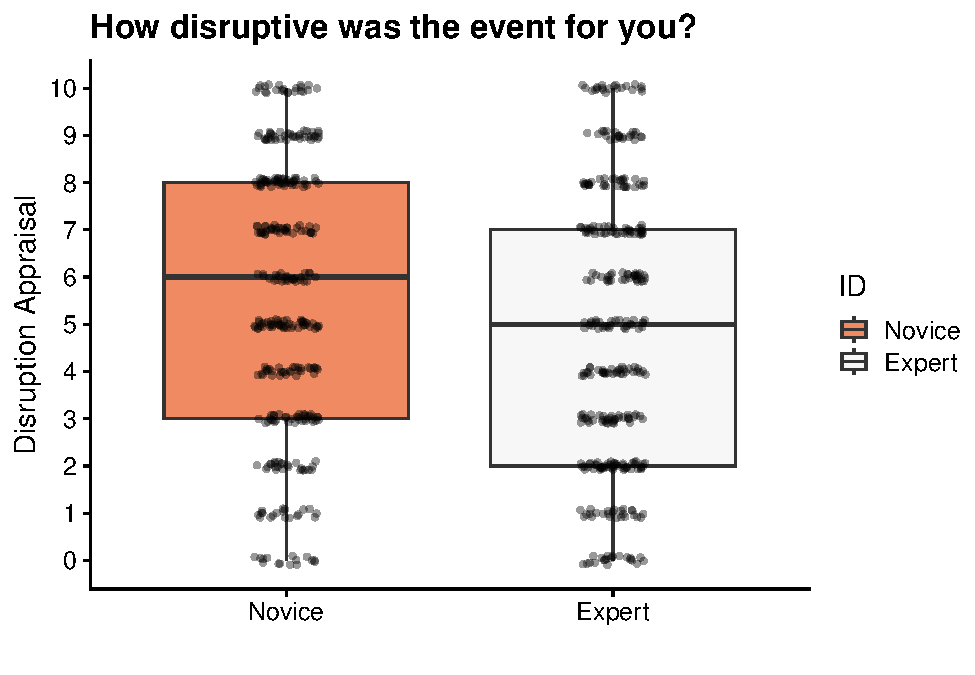
\includegraphics{expertise_2024_09_26_no_outlierdetection_MK_files/figure-latex/rating_scales-1.pdf}

\paragraph{t-Test \& effect size ``Disruption
appraisal''}\label{t-test-effect-size-disruption-appraisal}

\begin{verbatim}
Two Sample t-test
\end{verbatim}

data: sri\(disruption_appraisal[sri\)ID == ``Expert''{]} and
sri\(disruption_appraisal[sri\)ID == ``Novice''{]} t = -3.3143, df =
707, p-value = 0.0009655 alternative hypothesis: true difference in
means is not equal to 0 95 percent confidence interval: -1.1320397
-0.2897835 sample estimates: mean of x mean of y 4.840909 5.551821

{[}1{]} -0.25 attr(,``magnitude'') {[}1{]} ``small''

\begin{longtable}[]{@{}lrrrr@{}}
\caption{Confidence appraisal}\tabularnewline
\toprule\noalign{}
ID & M & SD & Min & Max \\
\midrule\noalign{}
\endfirsthead
\toprule\noalign{}
ID & M & SD & Min & Max \\
\midrule\noalign{}
\endhead
\bottomrule\noalign{}
\endlastfoot
Expert & 8.42 & 1.70 & 2 & 10 \\
Novice & 7.18 & 2.04 & 0 & 10 \\
\end{longtable}

\begin{longtable}[]{@{}llrrrrr@{}}
\caption{Confidence appraisal with event}\tabularnewline
\toprule\noalign{}
ID & event & N & M & SD & Min & Max \\
\midrule\noalign{}
\endfirsthead
\toprule\noalign{}
ID & event & N & M & SD & Min & Max \\
\midrule\noalign{}
\endhead
\bottomrule\noalign{}
\endlastfoot
Expert & chatting & 41 & 8.10 & 1.76 & 2 & 10 \\
Expert & clicking pen & 38 & 8.50 & 1.25 & 5 & 10 \\
Expert & drawing & 35 & 9.23 & 1.00 & 5 & 10 \\
Expert & drumming & 39 & 8.74 & 1.21 & 6 & 10 \\
Expert & head on table & 40 & 8.72 & 1.22 & 5 & 10 \\
Expert & heckling & 41 & 6.78 & 2.41 & 2 & 10 \\
Expert & looking at phone & 36 & 8.75 & 1.44 & 4 & 10 \\
Expert & snipping & 41 & 8.83 & 1.60 & 4 & 10 \\
Expert & whispering & 41 & 8.32 & 1.71 & 3 & 10 \\
Novice & chatting & 42 & 6.69 & 1.97 & 0 & 10 \\
Novice & clicking pen & 40 & 7.40 & 1.72 & 3 & 10 \\
Novice & drawing & 35 & 8.63 & 1.29 & 5 & 10 \\
Novice & drumming & 40 & 7.32 & 2.12 & 1 & 10 \\
Novice & head on table & 40 & 7.03 & 1.78 & 3 & 10 \\
Novice & heckling & 41 & 5.41 & 2.55 & 1 & 10 \\
Novice & looking at phone & 35 & 7.34 & 1.59 & 3 & 10 \\
Novice & snipping & 42 & 8.02 & 1.63 & 3 & 10 \\
Novice & whispering & 42 & 7.05 & 1.91 & 2 & 10 \\
\end{longtable}

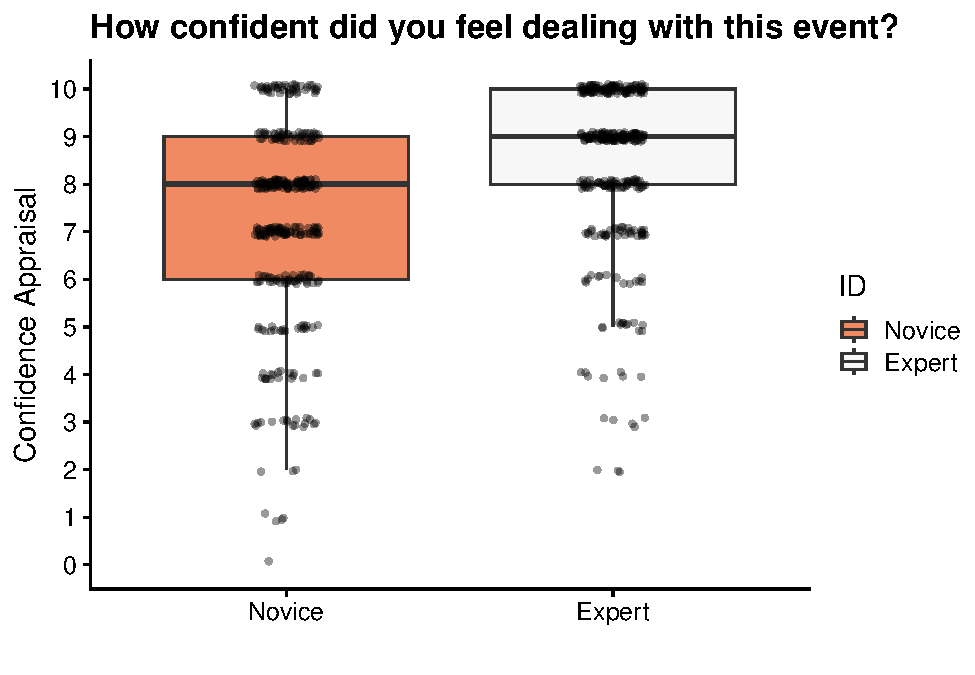
\includegraphics{expertise_2024_09_26_no_outlierdetection_MK_files/figure-latex/sri_ca-1.pdf}

\paragraph{t-Test \& effect size ``Confidence
appraisal''}\label{t-test-effect-size-confidence-appraisal}

\begin{verbatim}
Two Sample t-test
\end{verbatim}

data: sri\(confidence_appraisal[sri\)ID == ``Expert''{]} and
sri\(confidence_appraisal[sri\)ID == ``Novice''{]} t = 8.766, df = 707,
p-value \textless{} 2.2e-16 alternative hypothesis: true difference in
means is not equal to 0 95 percent confidence interval: 0.9588466
1.5123145 sample estimates: mean of x mean of y 8.420455 7.184874

{[}1{]} 0.66 attr(,``magnitude'') {[}1{]} ``medium''

\section{\texorpdfstring{\texttt{\{r\ sri\_pr,\ echo=FALSE,\ message=FALSE,\ warning=FALSE,\ results=\textquotesingle{}asis\textquotesingle{}\}\ \#\ \ \#\ \#\#\#\#\#\#\#\#\#\#\#\#\#\#\ Prevalence\ Rating\ \#\#\#\#\#\#\#\#\#\#\#\#\#\#\#\#\#\#\#\#\#\#\#\#\#\ \#\ \ \#\ sri.preva.table\ \textless{}-\ \#\ \ \ sri\ \%\textgreater{}\%\ \#\ \ \ group\_by(ID)\ \%\textgreater{}\%\ \#\ \ \ summarise(\ \#\ \ \ \ \ N\ =\ n(),\ \#\ \ \ \ \ "M"\ =\ round(mean(prevalence\_rating),\ digits\ =\ 2),\ \#\ \ \ \ \ "SD"\ =\ round(sd(prevalence\_rating),\ digits\ =\ 2),\ \#\ \ \ \ \ "Min"\ =\ min(prevalence\_rating),\ \#\ \ \ \ \ "Max"\ =\ max(prevalence\_rating)\ \#\ \ \ )\ \#\ \ \#\ \#\ insert\ a\ table\ into\ HTML\ \#\ knitr::kable(sri.preva.table,\ \#\ \ \ \ \ \ \ \ \ \ \ \ \ \ caption\ =\ "Prevalence\ rating")\ \#\ \ \#\ \#\#\#\#\ with\ event\ \ \#\ sri.preva.event.table\ \textless{}-\ \#\ \ \ sri\ \%\textgreater{}\%\ \#\ \ \ group\_by(ID,\ event)\ \%\textgreater{}\%\ \#\ \ \ summarise(\ \#\ \ \ \ \ N\ =\ n(),\ \#\ \ \ \ \ "M"\ =\ round(mean(prevalence\_rating),\ digits\ =\ 2),\ \#\ \ \ \ \ "SD"\ =\ round(sd(prevalence\_rating),\ digits\ =\ 2),\ \#\ \ \ \ \ "Min"\ =\ min(prevalence\_rating),\ \#\ \ \ \ \ "Max"\ =\ max(prevalence\_rating)\ \#\ \ \ )\ \#\ \ \#\ \#\ insert\ a\ table\ into\ HTML\ \#\ knitr::kable(sri.preva.event.table,\ \#\ \ \ \ \ \ \ \ \ \ \ \ \ \ caption\ =\ "Prevalence\ rating\ with\ events")\ \#\ \ \#\ \#\ create\ a\ new\ data\ frame\ with\ rating\ \#\ sri\_preva\ \textless{}-\ subset.data.frame(sri,\ select\ =\ c(ID,\ event,\ prevalence\_rating))\ \#\ \ \#\ \#\ plotting\ prevalence\ rating\ for\ groups\ \#\ preva\_group\_plot\ \textless{}-\ \ \#\ \ \ sri\_preva\ \%\textgreater{}\%\ \ \#\ \ \ mutate(ID\ =\ factor(ID,\ \#\ \ \ \ \ \ \ \ \ \ \ \ \ \ \ \ \ \ \ \ \ \ levels\ =\ c("Novice",\ \#\ \ \ \ \ \ \ \ \ \ \ \ \ \ \ \ \ \ \ \ \ \ \ \ \ \ \ \ \ \ \ \ \ "Expert"\ \#\ \ \ \ \ \ \ \ \ \ \ \ \ \ \ \ \ \ \ \ \ \ \ \ \ \ \ \ \ \ \ \ \ )\ \#\ \ \ \ \ \ \ \ \ \ \ \ \ \ \ \ \ \ \ \ \ \ )\ \#\ \ \ \ \ \ \ \ \ \ )\ \%\textgreater{}\%\ \ \#\ \ \ ggplot(mapping\ =\ aes(x\ =\ ID,\ \#\ \ \ \ \ \ \ \ \ \ \ \ \ \ \ \ \ \ \ \ \ \ \ \ y\ =\ prevalence\_rating))\ +\ \#\ \ \ geom\_boxplot(mapping\ =\ aes(fill\ =\ ID),\ \#\ \ \ \ \ \ \ \ \ \ \ \ \ \ \ \ outlier.shape\ =\ NA)\ +\ \#\ \ \ geom\_point(size\ =\ 1,\ \#\ \ \ \ \ \ \ \ \ \ \ \ \ \ alpha\ =\ 0.4,\ \#\ \ \ \ \ \ \ \ \ \ \ \ \ \ position\ =\ position\_jitter(seed\ =\ 1,\ \#\ \ \ \ \ \ \ \ \ \ \ \ \ \ \ \ \ \ \ \ \ \ \ \ \ \ \ \ \ \ \ \ \ \ \ \ \ \ \ \ \ width\ =\ 0.1,\ \#\ \ \ \ \ \ \ \ \ \ \ \ \ \ \ \ \ \ \ \ \ \ \ \ \ \ \ \ \ \ \ \ \ \ \ \ \ \ \ \ \ height\ =\ 0.1))\ +\ \#\ \ \ scale\_x\_discrete(limits\ =\ c("Novice",\ "Expert"))\ +\ \#\ \ \ scale\_y\_continuous(breaks\ =\ seq(from\ =\ 0,\ to\ =\ 10,\ by\ =\ 1))\ +\ \ \#\ \ \ labs(x\ =\ "",\ \#\ \ \ \ \ \ \ \ y\ =\ "Prevalence\ Rating")\ +\ \ \#\ \ \ scale\_fill\_brewer(palette\ \ =\ "RdBu")\ +\ \ \ \#\ \ \ ggtitle("How\ widespread\ is\ this\ event\ in\ the\ classroom?")\ +\ \#\ \ \ theme\_cowplot()\ \#\ \ \#\ preva\_group\_plot\ \#\ \ \#}}{\{r sri\_pr, echo=FALSE, message=FALSE, warning=FALSE, results=\textquotesingle asis\textquotesingle\} \#  \# \#\#\#\#\#\#\#\#\#\#\#\#\#\# Prevalence Rating \#\#\#\#\#\#\#\#\#\#\#\#\#\#\#\#\#\#\#\#\#\#\#\#\# \#  \# sri.preva.table \textless- \#   sri \%\textgreater\% \#   group\_by(ID) \%\textgreater\% \#   summarise( \#     N = n(), \#     "M" = round(mean(prevalence\_rating), digits = 2), \#     "SD" = round(sd(prevalence\_rating), digits = 2), \#     "Min" = min(prevalence\_rating), \#     "Max" = max(prevalence\_rating) \#   ) \#  \# \# insert a table into HTML \# knitr::kable(sri.preva.table, \#              caption = "Prevalence rating") \#  \# \#\#\#\# with event  \# sri.preva.event.table \textless- \#   sri \%\textgreater\% \#   group\_by(ID, event) \%\textgreater\% \#   summarise( \#     N = n(), \#     "M" = round(mean(prevalence\_rating), digits = 2), \#     "SD" = round(sd(prevalence\_rating), digits = 2), \#     "Min" = min(prevalence\_rating), \#     "Max" = max(prevalence\_rating) \#   ) \#  \# \# insert a table into HTML \# knitr::kable(sri.preva.event.table, \#              caption = "Prevalence rating with events") \#  \# \# create a new data frame with rating \# sri\_preva \textless- subset.data.frame(sri, select = c(ID, event, prevalence\_rating)) \#  \# \# plotting prevalence rating for groups \# preva\_group\_plot \textless-  \#   sri\_preva \%\textgreater\%  \#   mutate(ID = factor(ID, \#                      levels = c("Novice", \#                                 "Expert" \#                                 ) \#                      ) \#          ) \%\textgreater\%  \#   ggplot(mapping = aes(x = ID, \#                        y = prevalence\_rating)) + \#   geom\_boxplot(mapping = aes(fill = ID), \#                outlier.shape = NA) + \#   geom\_point(size = 1, \#              alpha = 0.4, \#              position = position\_jitter(seed = 1, \#                                         width = 0.1, \#                                         height = 0.1)) + \#   scale\_x\_discrete(limits = c("Novice", "Expert")) + \#   scale\_y\_continuous(breaks = seq(from = 0, to = 10, by = 1)) +  \#   labs(x = "", \#        y = "Prevalence Rating") +  \#   scale\_fill\_brewer(palette  = "RdBu") +   \#   ggtitle("How widespread is this event in the classroom?") + \#   theme\_cowplot() \#  \# preva\_group\_plot \#  \#}}\label{r-sri_pr-echofalse-messagefalse-warningfalse-resultsasis-prevalence-rating-sri.preva.table---sri-group_byid-summarise-n-n-m-roundmeanprevalence_rating-digits-2-sd-roundsdprevalence_rating-digits-2-min-minprevalence_rating-max-maxprevalence_rating-insert-a-table-into-html-knitrkablesri.preva.table-caption-prevalence-rating-with-event-sri.preva.event.table---sri-group_byid-event-summarise-n-n-m-roundmeanprevalence_rating-digits-2-sd-roundsdprevalence_rating-digits-2-min-minprevalence_rating-max-maxprevalence_rating-insert-a-table-into-html-knitrkablesri.preva.event.table-caption-prevalence-rating-with-events-create-a-new-data-frame-with-rating-sri_preva---subset.data.framesri-select-cid-event-prevalence_rating-plotting-prevalence-rating-for-groups-preva_group_plot---sri_preva-mutateid-factorid-levels-cnovice-expert-ggplotmapping-aesx-id-y-prevalence_rating-geom_boxplotmapping-aesfill-id-outlier.shape-na-geom_pointsize-1-alpha-0.4-position-position_jitterseed-1-width-0.1-height-0.1-scale_x_discretelimits-cnovice-expert-scale_y_continuousbreaks-seqfrom-0-to-10-by-1-labsx-y-prevalence-rating-scale_fill_brewerpalette-rdbu-ggtitlehow-widespread-is-this-event-in-the-classroom-theme_cowplot-preva_group_plot}

\paragraph{t-Test \& effect size ``Prevalence
rating''}\label{t-test-effect-size-prevalence-rating}

\section{\texorpdfstring{\texttt{\{r\ sri\_pr\_ttest,\ echo=FALSE,\ message=FALSE,\ warning=FALSE,\ results=\textquotesingle{}asis\textquotesingle{}\}\ \#\ \ \#\ \#\#\#\#\#\#\#\#\#\#\#\#\#\#\#\#\#\#\#\#\ T-TEST\ \&\ EFFECT\ SIZE\ \#\#\#\#\#\#\#\#\#\#\#\#\ \#\ \ \#\ \#\ Prevalence\ Rating\ \ \#\ \#\ t-test\ for\ expertise\ differences\ \#\ t.test(x\ =\ sri\$prevalence\_rating{[}sri\$ID\ ==\ "Expert"{]},\ \#\ \ \ \ \ \ \ \ y\ =\ sri\$prevalence\_rating{[}sri\$ID\ ==\ "Novice"{]},\ \#\ \ \ \ \ \ \ \ var.equal\ =\ TRUE)\ \#\ \ \#\ \#\ Prevalence\ Rating\ \ \#\ \#\ effect\ size\ for\ expertise\ differences\ \#\ d\_sri\_preva\ \textless{}-\ CohenD(x\ =\ sri\$prevalence\_rating{[}sri\$ID\ ==\ "Expert"{]},\ \#\ \ \ \ \ \ \ \ \ \ \ \ \ \ \ \ \ \ \ \ \ \ \ y\ =\ sri\$prevalence\_rating{[}sri\$ID\ ==\ "Novice"{]},\ \#\ \ \ \ \ \ \ \ \ \ \ \ \ \ \ \ \ \ \ \ \ \ \ na.rm\ =\ TRUE)\ \#\ \ \#\ round(d\_sri\_preva,\ 2)\ \#\ \ \#}}{\{r sri\_pr\_ttest, echo=FALSE, message=FALSE, warning=FALSE, results=\textquotesingle asis\textquotesingle\} \#  \# \#\#\#\#\#\#\#\#\#\#\#\#\#\#\#\#\#\#\#\# T-TEST \& EFFECT SIZE \#\#\#\#\#\#\#\#\#\#\#\# \#  \# \# Prevalence Rating  \# \# t-test for expertise differences \# t.test(x = sri\$prevalence\_rating{[}sri\$ID == "Expert"{]}, \#        y = sri\$prevalence\_rating{[}sri\$ID == "Novice"{]}, \#        var.equal = TRUE) \#  \# \# Prevalence Rating  \# \# effect size for expertise differences \# d\_sri\_preva \textless- CohenD(x = sri\$prevalence\_rating{[}sri\$ID == "Expert"{]}, \#                       y = sri\$prevalence\_rating{[}sri\$ID == "Novice"{]}, \#                       na.rm = TRUE) \#  \# round(d\_sri\_preva, 2) \#  \#}}\label{r-sri_pr_ttest-echofalse-messagefalse-warningfalse-resultsasis-t-test-effect-size-prevalence-rating-t-test-for-expertise-differences-t.testx-sriprevalence_ratingsriid-expert-y-sriprevalence_ratingsriid-novice-var.equal-true-prevalence-rating-effect-size-for-expertise-differences-d_sri_preva---cohendx-sriprevalence_ratingsriid-expert-y-sriprevalence_ratingsriid-novice-na.rm-true-roundd_sri_preva-2}

\subsubsection{Internal consistency (Omega) for disruption and
confidence
appraisal}\label{internal-consistency-omega-for-disruption-and-confidence-appraisal}

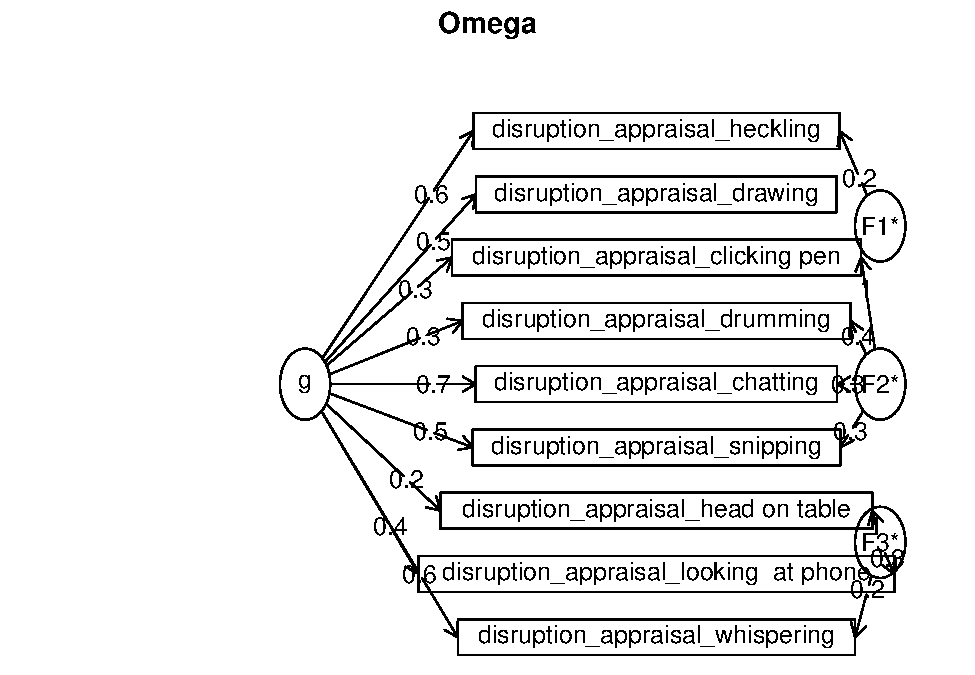
\includegraphics{expertise_2024_09_26_no_outlierdetection_MK_files/figure-latex/sri_omega-1.pdf}
Omega Call: omegah(m = m, nfactors = nfactors, fm = fm, key = key, flip
= flip, digits = digits, title = title, sl = sl, labels = labels, plot =
plot, n.obs = n.obs, rotate = rotate, Phi = Phi, option = option, covar
= covar) Alpha: 0.76 G.6: 0.81 Omega Hierarchical: 0.62 Omega H
asymptotic: 0.73 Omega Total 0.84

Schmid Leiman Factor loadings greater than 0.2 g F1* F2* F3* h2 h2 u2
disruption\_appraisal\_whispering 0.60 0.22 0.45 0.45 0.55
disruption\_appraisal\_heckling 0.63 0.24 0.47 0.47 0.53
disruption\_appraisal\_drawing 0.47 0.27 0.27 0.73
disruption\_appraisal\_snipping 0.50 0.26 0.35 0.35 0.65
disruption\_appraisal\_looking at phone 0.38 0.32 0.26 0.26 0.74
disruption\_appraisal\_head on table 0.22 0.98 1.00 1.00 0.00
disruption\_appraisal\_clicking pen 0.34 0.95 1.02 1.02 -0.02
disruption\_appraisal\_drumming 0.34 0.37 0.28 0.28 0.72
disruption\_appraisal\_chatting 0.67 0.28 0.57 0.57 0.43 p2 com
disruption\_appraisal\_whispering 0.80 1.52
disruption\_appraisal\_heckling 0.84 1.39 disruption\_appraisal\_drawing
0.82 1.45 disruption\_appraisal\_snipping 0.71 1.85
disruption\_appraisal\_looking at phone 0.57 2.12
disruption\_appraisal\_head on table 0.05 1.10
disruption\_appraisal\_clicking pen 0.11 1.25
disruption\_appraisal\_drumming 0.42 2.35
disruption\_appraisal\_chatting 0.80 1.52

With Sums of squares of: g F1* F2* F3* h2 2.10 0.19 1.22 1.16 3.13

general/max 0.67 max/min = 16.24 mean percent general = 0.57 with sd =
0.31 and cv of 0.54 Explained Common Variance of the general factor =
0.45

The degrees of freedom are 12 and the fit is 0.35 The number of
observations was 53 with Chi Square = 16.18 with prob \textless{} 0.18
The root mean square of the residuals is 0.05 The df corrected root mean
square of the residuals is 0.09 RMSEA index = 0.079 and the 10 \%
confidence intervals are 0 0.174 BIC = -31.47

Compare this with the adequacy of just a general factor and no group
factors The degrees of freedom for just the general factor are 27 and
the fit is 1.18 The number of observations was 53 with Chi Square = 56
with prob \textless{} 0.00086 The root mean square of the residuals is
0.13 The df corrected root mean square of the residuals is 0.16

RMSEA index = 0.141 and the 10 \% confidence intervals are 0.09 0.197
BIC = -51.2

Measures of factor score adequacy\\
g F1* F2* F3* Correlation of scores with factors 0.84 0.30 1.01 1.00
Multiple R square of scores with factors 0.70 0.09 1.02 0.99 Minimum
correlation of factor score estimates 0.41 -0.82 1.03 0.99

Total, General and Subset omega for each subset g F1* F2* F3* Omega
total for total scores and subscales 0.84 0.54 0.79 0.72 Omega general
for total scores and subscales 0.62 0.47 0.39 0.28 Omega group for total
scores and subscales 0.21 0.06 0.39 0.44
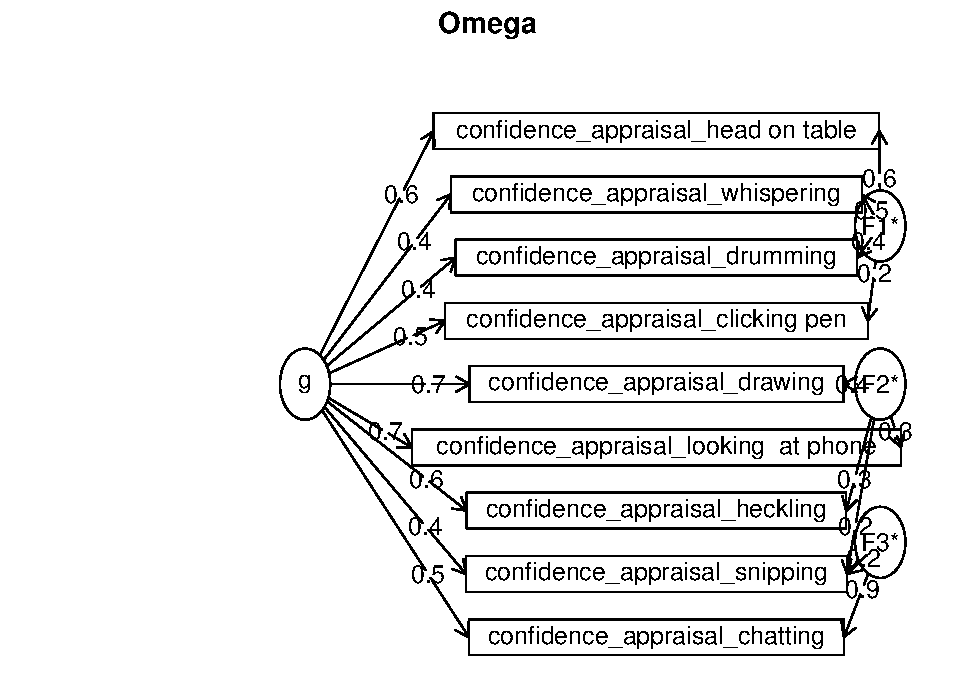
\includegraphics{expertise_2024_09_26_no_outlierdetection_MK_files/figure-latex/sri_omega-2.pdf}
Omega Call: omegah(m = m, nfactors = nfactors, fm = fm, key = key, flip
= flip, digits = digits, title = title, sl = sl, labels = labels, plot =
plot, n.obs = n.obs, rotate = rotate, Phi = Phi, option = option, covar
= covar) Alpha: 0.82 G.6: 0.84 Omega Hierarchical: 0.66 Omega H
asymptotic: 0.76 Omega Total 0.87

Schmid Leiman Factor loadings greater than 0.2 g F1* F2* F3* h2 h2 u2
confidence\_appraisal\_whispering 0.39 0.48 0.40 0.40 0.60
confidence\_appraisal\_heckling 0.59 0.28 0.45 0.45 0.55
confidence\_appraisal\_drawing 0.70 0.36 0.62 0.62 0.38
confidence\_appraisal\_snipping 0.41 0.23 0.23 0.31 0.31 0.69
confidence\_appraisal\_looking at phone 0.66 0.32 0.57 0.57 0.43
confidence\_appraisal\_head on table 0.56 0.56 0.63 0.63 0.37
confidence\_appraisal\_clicking pen 0.48 0.20 0.31 0.31 0.69
confidence\_appraisal\_drumming 0.42 0.42 0.37 0.37 0.63
confidence\_appraisal\_chatting 0.50 0.87 1.00 1.00 0.00 p2 com
confidence\_appraisal\_whispering 0.38 2.11
confidence\_appraisal\_heckling 0.76 1.62 confidence\_appraisal\_drawing
0.79 1.50 confidence\_appraisal\_snipping 0.55 2.69
confidence\_appraisal\_looking at phone 0.75 1.67
confidence\_appraisal\_head on table 0.50 2.03
confidence\_appraisal\_clicking pen 0.74 1.74
confidence\_appraisal\_drumming 0.49 2.10
confidence\_appraisal\_chatting 0.25 1.60

With Sums of squares of: g F1* F2* F3* h2 2.55 0.82 0.39 0.90 2.80

general/max 0.91 max/min = 7.18 mean percent general = 0.58 with sd =
0.19 and cv of 0.33 Explained Common Variance of the general factor =
0.55

The degrees of freedom are 12 and the fit is 0.33 The number of
observations was 53 with Chi Square = 15.22 with prob \textless{} 0.23
The root mean square of the residuals is 0.05 The df corrected root mean
square of the residuals is 0.09 RMSEA index = 0.069 and the 10 \%
confidence intervals are 0 0.167 BIC = -32.43

Compare this with the adequacy of just a general factor and no group
factors The degrees of freedom for just the general factor are 27 and
the fit is 0.87 The number of observations was 53 with Chi Square = 41.5
with prob \textless{} 0.037 The root mean square of the residuals is
0.12 The df corrected root mean square of the residuals is 0.14

RMSEA index = 0.099 and the 10 \% confidence intervals are 0.026 0.16
BIC = -65.7

Measures of factor score adequacy\\
g F1* F2* F3* Correlation of scores with factors 0.84 0.72 0.48 0.96
Multiple R square of scores with factors 0.70 0.52 0.23 0.92 Minimum
correlation of factor score estimates 0.41 0.04 -0.55 0.83

Total, General and Subset omega for each subset g F1* F2* F3* Omega
total for total scores and subscales 0.87 0.71 0.77 1.00 Omega general
for total scores and subscales 0.66 0.40 0.61 0.25 Omega group for total
scores and subscales 0.15 0.32 0.16 0.75

\subsubsection{Prevalence Rating as manipulation
check}\label{prevalence-rating-as-manipulation-check}

\subsubsection{2.3 Situational Jugdement
Test}\label{situational-jugdement-test}

\begin{longtable}[]{@{}lrrrrr@{}}
\caption{N, M and SD for overall value}\tabularnewline
\toprule\noalign{}
Group & N & M & SD & Min & Max \\
\midrule\noalign{}
\endfirsthead
\toprule\noalign{}
Group & N & M & SD & Min & Max \\
\midrule\noalign{}
\endhead
\bottomrule\noalign{}
\endlastfoot
Expert & 41 & 0.75 & 0.08 & 0.54 & 0.88 \\
Novice & 42 & 0.72 & 0.13 & 0.10 & 0.91 \\
\end{longtable}

\begin{longtable}[]{@{}lrrrrr@{}}
\caption{N, M and SD for managing momentum}\tabularnewline
\toprule\noalign{}
Group & N & M & SD & Min & Max \\
\midrule\noalign{}
\endfirsthead
\toprule\noalign{}
Group & N & M & SD & Min & Max \\
\midrule\noalign{}
\endhead
\bottomrule\noalign{}
\endlastfoot
Expert & 41 & 0.81 & 0.10 & 0.60 & 1 \\
Novice & 42 & 0.80 & 0.17 & 0.08 & 1 \\
\end{longtable}

\begin{longtable}[]{@{}lrrrrr@{}}
\caption{N, M and SD for monitoring}\tabularnewline
\toprule\noalign{}
Group & N & M & SD & Min & Max \\
\midrule\noalign{}
\endfirsthead
\toprule\noalign{}
Group & N & M & SD & Min & Max \\
\midrule\noalign{}
\endhead
\bottomrule\noalign{}
\endlastfoot
Expert & 41 & 0.69 & 0.13 & 0.41 & 0.91 \\
Novice & 42 & 0.64 & 0.16 & 0.15 & 0.99 \\
\end{longtable}

\begin{longtable}[]{@{}lrrrrr@{}}
\caption{N, M and SD for rules and routines}\tabularnewline
\toprule\noalign{}
Group & N & M & SD & Min & Max \\
\midrule\noalign{}
\endfirsthead
\toprule\noalign{}
Group & N & M & SD & Min & Max \\
\midrule\noalign{}
\endhead
\bottomrule\noalign{}
\endlastfoot
Expert & 41 & 0.74 & 0.10 & 0.49 & 0.91 \\
Novice & 42 & 0.72 & 0.13 & 0.07 & 0.92 \\
\end{longtable}

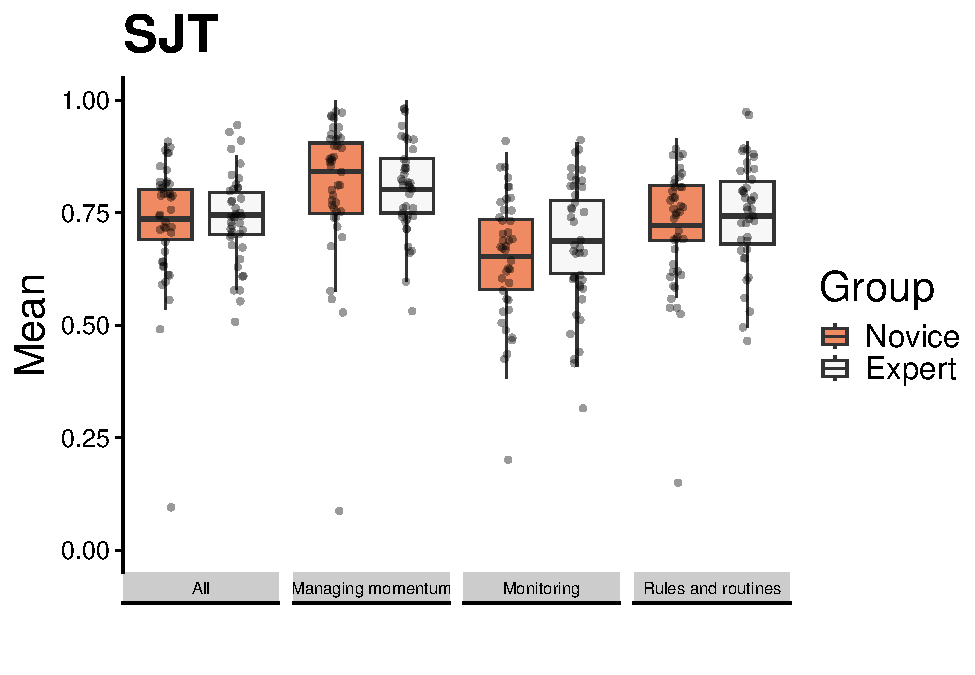
\includegraphics{expertise_2024_09_26_no_outlierdetection_MK_files/figure-latex/sjt-1.pdf}

\paragraph{t-test \& effect size ``STJ -
All''}\label{t-test-effect-size-stj---all}

\begin{verbatim}
Two Sample t-test
\end{verbatim}

data: df\_sjt\(All[df_sjt\)Group == ``Expert''{]} and
df\_sjt\(All[df_sjt\)Group == ``Novice''{]} t = 0.94245, df = 81,
p-value = 0.3488 alternative hypothesis: true difference in means is not
equal to 0 95 percent confidence interval: -0.02434447 0.06816136 sample
estimates: mean of x mean of y 0.7456548 0.7237464

{[}1{]} 0.21 attr(,``magnitude'') {[}1{]} ``small''

\paragraph{t-test \& effect size ``SJT - Managing
momentum''}\label{t-test-effect-size-sjt---managing-momentum}

\begin{verbatim}
Two Sample t-test
\end{verbatim}

data: df\_sjt\(`Managing momentum`[df_sjt\)Group == ``Expert''{]} and
df\_sjt\(`Managing momentum`[df_sjt\)Group == ``Novice''{]} t = 0.15193,
df = 81, p-value = 0.8796 alternative hypothesis: true difference in
means is not equal to 0 95 percent confidence interval: -0.05469659
0.06374016 sample estimates: mean of x mean of y 0.8092270 0.8047052

{[}1{]} 0.03 attr(,``magnitude'') {[}1{]} ``negligible''

\paragraph{t-test \& effect size ``SJT -
Monitoring''}\label{t-test-effect-size-sjt---monitoring}

\begin{verbatim}
Two Sample t-test
\end{verbatim}

data: df\_sjt\(Monitoring[df_sjt\)Group == ``Expert''{]} and
df\_sjt\(Monitoring[df_sjt\)Group == ``Novice''{]} t = 1.4415, df = 81,
p-value = 0.1533 alternative hypothesis: true difference in means is not
equal to 0 95 percent confidence interval: -0.01732034 0.10841421 sample
estimates: mean of x mean of y 0.6877186 0.6421717

{[}1{]} 0.32 attr(,``magnitude'') {[}1{]} ``small''

\paragraph{t-test \& effect size ``SJT - Rules \&
routines''}\label{t-test-effect-size-sjt---rules-routines}

\begin{verbatim}
Two Sample t-test
\end{verbatim}

data: df\_sjt\(`Rules and routines`[df_sjt\)Group == ``Expert''{]} and
df\_sjt\(`Rules and routines`[df_sjt\)Group == ``Novice''{]} t =
0.59927, df = 81, p-value = 0.5507 alternative hypothesis: true
difference in means is not equal to 0 95 percent confidence interval:
-0.03632644 0.06763970 sample estimates: mean of x mean of y 0.7400189
0.7243622

{[}1{]} 0.13 attr(,``magnitude'') {[}1{]} ``negligible''

\subsubsection{Internal consistency (Omega) for
SJT}\label{internal-consistency-omega-for-sjt}

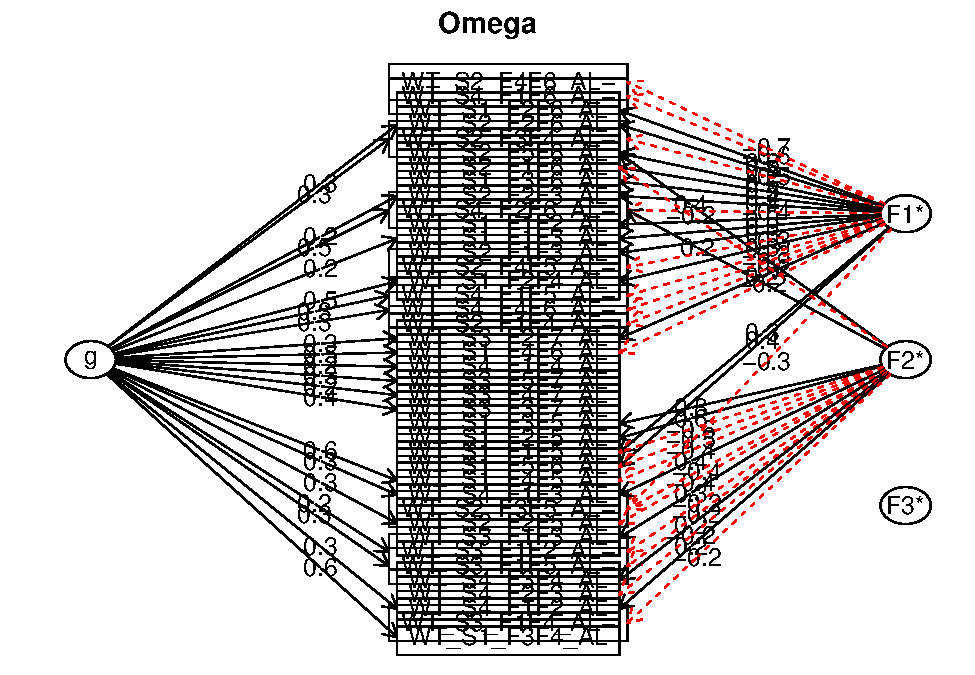
\includegraphics{expertise_2024_09_26_no_outlierdetection_MK_files/figure-latex/sjt_omega-1.pdf}
Omega Call: omegah(m = m, nfactors = nfactors, fm = fm, key = key, flip
= flip, digits = digits, title = title, sl = sl, labels = labels, plot =
plot, n.obs = n.obs, rotate = rotate, Phi = Phi, option = option, covar
= covar) Alpha: 0.68 G.6: 0.9 Omega Hierarchical: 0.66 Omega H
asymptotic: 0.88 Omega Total 0.75

Schmid Leiman Factor loadings greater than 0.2 g F1* F2* F3* h2 h2 u2 p2
com WT\_S1\_F1F2\_AL 0.35 0.15 0.85 0.13 1.47 WT\_S1\_F1F3\_AL 0.25 0.33
0.19 0.81 0.32 2.20 WT\_S1\_F1F5\_AL 0.26 -0.55 0.38 0.38 0.62 0.04 1.54
WT\_S1\_F2F4\_AL 0.49 0.31 0.35 0.35 0.65 0.69 1.81 WT\_S1\_F2F5\_AL
0.63 0.42 0.42 0.58 0.00 1.13 WT\_S1\_F2F6\_AL 0.57 0.35 0.35 0.65 0.01
1.16 WT\_S1\_F3F4\_AL 0.57 0.36 0.36 0.64 0.90 1.21 WT\_S1\_F3F5\_AL
0.78 0.61 0.61 0.39 0.00 1.02 WT\_S1\_F3F6\_AL 0.44 0.23 0.23 0.77 0.05
1.33 WT\_S1\_F4F5\_AL 0.60 -0.39 0.52 0.52 0.48 0.69 1.75
WT\_S1\_F4F6\_AL 0.47 -0.20 0.27 0.27 0.73 0.84 1.38 WT\_S1\_F5F6\_AL
0.42 -0.50 0.45 0.45 0.55 0.07 2.20 WT\_S2\_F1F3\_AL 0.33 0.14 0.86 0.02
1.52 WT\_S2\_F1F4\_AL- -0.24 0.10 0.90 0.07 2.13 WT\_S2\_F1F6\_AL 0.49
-0.24 0.32 0.32 0.68 0.11 1.78 WT\_S2\_F2F3\_AL 0.22 0.44 0.24 0.24 0.76
0.20 1.48 WT\_S2\_F2F5\_AL 0.32 -0.35 0.23 0.23 0.77 0.45 2.06
WT\_S2\_F2F6\_AL 0.26 0.54 0.37 0.37 0.63 0.19 1.48 WT\_S2\_F3F4\_AL-
0.31 -0.52 0.38 0.38 0.62 0.26 1.66 WT\_S2\_F3F5\_AL- -0.33 -0.35 0.26
0.26 0.74 0.09 2.37 WT\_S2\_F4F5\_AL- -0.31 0.15 0.85 0.14 2.13
WT\_S2\_F4F6\_AL- -0.69 0.48 0.48 0.52 0.01 1.01 WT\_S2\_F5F6\_AL 0.51
0.38 0.42 0.42 0.58 0.01 1.89 WT\_S3\_F1F2\_AL- 0.25 -0.24 0.13 0.87
0.50 2.14 WT\_S3\_F1F3\_AL 0.32 0.12 0.88 0.11 1.31 WT\_S3\_F1F4\_AL-
-0.20 0.05 0.95 0.04 1.27 WT\_S3\_F1F5\_AL- 0.26 -0.24 0.13 0.87 0.54
2.02 WT\_S3\_F2F7\_AL 0.31 0.21 0.16 0.84 0.57 2.37 WT\_S3\_F3F7\_AL
0.38 0.15 0.85 0.94 1.13 WT\_S3\_F4F7\_AL 0.24 0.06 0.94 0.86 1.33
WT\_S3\_F5F7\_AL 0.34 0.13 0.87 0.89 1.24 WT\_S4\_F1F2\_AL 0.29 0.21
0.16 0.84 0.53 2.49 WT\_S4\_F1F3\_AL 0.30 0.36 0.23 0.23 0.77 0.38 2.21
WT\_S4\_F1F4\_AL 0.20 0.06 0.94 0.64 1.86 WT\_S4\_F1F5\_AL- 0.27 -0.29
0.16 0.84 0.46 2.10 WT\_S4\_F1F6\_AL- -0.63 0.43 0.43 0.57 0.08 1.18
WT\_S4\_F2F3\_AL -0.22 0.06 0.94 0.07 1.50 WT\_S4\_F2F6\_AL- 0.47 -0.35
0.24 0.40 0.40 0.60 0.56 2.40 WT\_S4\_F3F4\_AL 0.23 0.06 0.94 0.00 1.08
WT\_S4\_F4F6\_AL- 0.26 -0.26 0.14 0.86 0.49 2.10

With Sums of squares of: g F1* F2* F3* h2 2.88 4.10 3.00 0.01 3.35

general/max 0.7 max/min = 293.69 mean percent general = 0.32 with sd =
0.31 and cv of 0.95 Explained Common Variance of the general factor =
0.29

The degrees of freedom are 663 and the fit is 18.76 The number of
observations was 84 with Chi Square = 1253.73 with prob \textless{}
6.8e-39 The root mean square of the residuals is 0.11 The df corrected
root mean square of the residuals is 0.12 RMSEA index = 0.102 and the 10
\% confidence intervals are 0.095 0.112 BIC = -1683.9

Compare this with the adequacy of just a general factor and no group
factors The degrees of freedom for just the general factor are 740 and
the fit is 24.06 The number of observations was 84 with Chi Square =
1639.81 with prob \textless{} 5e-70 The root mean square of the
residuals is 0.17 The df corrected root mean square of the residuals is
0.17

RMSEA index = 0.12 and the 10 \% confidence intervals are 0.113 0.129
BIC = -1639

Measures of factor score adequacy\\
g F1* F2* F3* Correlation of scores with factors 0.90 0.93 0.92 0.06
Multiple R square of scores with factors 0.81 0.87 0.84 0.00 Minimum
correlation of factor score estimates 0.62 0.73 0.69 -0.99

Total, General and Subset omega for each subset g F1* F2* F3* Omega
total for total scores and subscales 0.75 0.56 0.39 NA Omega general for
total scores and subscales 0.66 0.53 0.38 NA Omega group for total
scores and subscales 0.01 0.03 0.00 NA
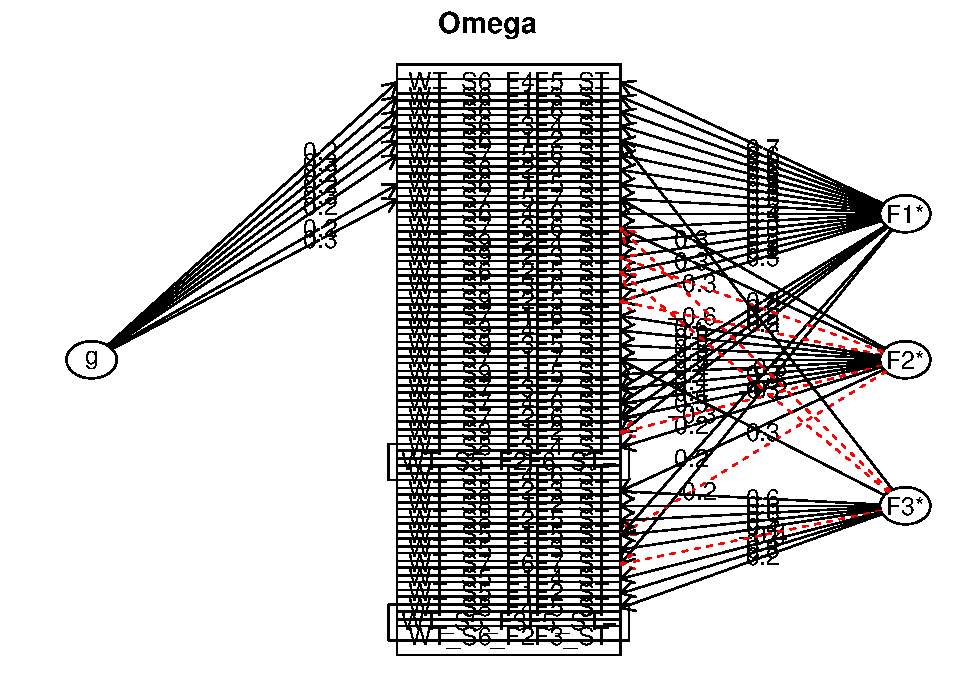
\includegraphics{expertise_2024_09_26_no_outlierdetection_MK_files/figure-latex/sjt_omega-2.pdf}
Omega Call: omegah(m = m, nfactors = nfactors, fm = fm, key = key, flip
= flip, digits = digits, title = title, sl = sl, labels = labels, plot =
plot, n.obs = n.obs, rotate = rotate, Phi = Phi, option = option, covar
= covar) Alpha: 0.81 G.6: 0.95 Omega Hierarchical: 0.13 Omega H
asymptotic: 0.16 Omega Total 0.84

Schmid Leiman Factor loadings greater than 0.2 g F1* F2* F3* h2 h2 u2 p2
com WT\_S5\_F1F2\_ST 0.28 0.11 0.89 0.09 1.90 WT\_S5\_F1F3\_ST 0.41 0.20
0.20 0.80 0.07 1.46 WT\_S5\_F1F4\_ST 0.37 0.19 0.81 0.06 1.74
WT\_S5\_F1F5\_ST 0.27 -0.22 0.53 0.42 0.42 0.58 0.05 2.08
WT\_S5\_F2F6\_ST- 0.04 0.96 0.00 1.68 WT\_S5\_F3F5\_ST- 0.20 0.08 0.92
0.02 2.57 WT\_S5\_F3F6\_ST 0.20 0.05 0.95 0.10 1.30 WT\_S5\_F4F6\_ST
0.05 0.95 0.14 2.61 WT\_S6\_F1F2\_ST 0.26 0.55 0.34 0.49 0.49 0.51 0.13
2.15 WT\_S6\_F1F3\_ST 0.25 0.64 0.50 0.50 0.50 0.13 1.44
WT\_S6\_F1F5\_ST 0.23 0.51 0.34 0.34 0.66 0.15 1.61 WT\_S6\_F1F6\_ST
0.25 0.64 0.48 0.48 0.52 0.13 1.35 WT\_S6\_F2F3\_ST 0.07 0.93 0.02 2.50
WT\_S6\_F2F4\_ST 0.55 0.35 0.35 0.65 0.09 1.34 WT\_S6\_F2F5\_ST 0.24
-0.21 0.13 0.87 0.05 2.87 WT\_S6\_F3F4\_ST 0.22 0.62 0.45 0.45 0.55 0.11
1.39 WT\_S6\_F4F5\_ST 0.25 0.71 0.58 0.58 0.42 0.10 1.32
WT\_S6\_F4F6\_ST 0.43 0.21 0.21 0.79 0.11 1.33 WT\_S7\_F1F6\_ST 0.64
0.48 0.48 0.52 0.07 1.37 WT\_S7\_F1F7\_ST 0.47 0.30 0.35 0.35 0.65 0.08
2.09 WT\_S7\_F2F6\_ST 0.24 0.29 0.17 0.83 0.09 2.78 WT\_S7\_F3F6\_ST
0.32 0.30 -0.30 0.30 0.30 0.70 0.06 3.30 WT\_S7\_F3F7\_ST 0.23 0.37 0.24
0.24 0.76 0.07 2.42 WT\_S7\_F4F6\_ST 0.30 0.37 0.28 0.28 0.72 0.08 2.78
WT\_S7\_F5F6\_ST 0.21 0.55 0.37 0.37 0.63 0.12 1.49 WT\_S7\_F5F7\_ST
0.25 0.46 0.31 0.39 0.39 0.61 0.16 2.64 WT\_S7\_F6F7\_ST 0.27 -0.37 0.23
0.23 0.77 0.02 2.02 WT\_S8\_F1F2\_ST 0.59 0.37 0.37 0.63 0.00 1.13
WT\_S8\_F2F3\_ST 0.24 0.63 0.47 0.47 0.53 0.03 1.37 WT\_S8\_F2F5\_ST
0.58 0.35 0.35 0.65 0.03 1.09 WT\_S8\_F3F4\_ST 0.22 0.05 0.95 0.04 1.21
WT\_S8\_F4F5\_ST 0.23 0.08 0.92 0.10 2.24 WT\_S9\_F1F2\_ST 0.24 -0.25
0.12 0.88 0.02 2.07 WT\_S9\_F1F5\_ST 0.41 0.19 0.81 0.06 1.36
WT\_S9\_F2F3\_ST 0.28 -0.27 0.16 0.84 0.03 2.14 WT\_S9\_F2F4\_ST 0.32
0.15 0.85 0.10 1.97 WT\_S9\_F2F5\_ST 0.35 -0.64 0.53 0.53 0.47 0.00 1.55
WT\_S9\_F3F5\_ST 0.48 0.27 0.27 0.73 0.01 1.33 WT\_S9\_F4F5\_ST 0.54
0.35 0.35 0.65 0.06 1.42

With Sums of squares of: g F1* F2* F3* h2 0.82 4.38 2.79 2.65 3.86

general/max 0.19 max/min = 1.65 mean percent general = 0.07 with sd =
0.04 and cv of 0.63 Explained Common Variance of the general factor =
0.08

The degrees of freedom are 627 and the fit is 18.95 The number of
observations was 84 with Chi Square = 1273.13 with prob \textless{}
2.9e-46 The root mean square of the residuals is 0.11 The df corrected
root mean square of the residuals is 0.12 RMSEA index = 0.11 and the 10
\% confidence intervals are 0.103 0.12 BIC = -1504.99

Compare this with the adequacy of just a general factor and no group
factors The degrees of freedom for just the general factor are 702 and
the fit is 24.66 The number of observations was 84 with Chi Square =
1689.12 with prob \textless{} 4.7e-83 The root mean square of the
residuals is 0.18 The df corrected root mean square of the residuals is
0.19

RMSEA index = 0.129 and the 10 \% confidence intervals are 0.122 0.138
BIC = -1421.31

Measures of factor score adequacy\\
g F1* F2* F3* Correlation of scores with factors 0.39 0.89 0.90 0.89
Multiple R square of scores with factors 0.15 0.80 0.81 0.80 Minimum
correlation of factor score estimates -0.70 0.60 0.61 0.59

Total, General and Subset omega for each subset g F1* F2* F3* Omega
total for total scores and subscales 0.84 0.84 0.39 0.49 Omega general
for total scores and subscales 0.13 0.11 0.06 0.04 Omega group for total
scores and subscales 0.37 0.73 0.33 0.45
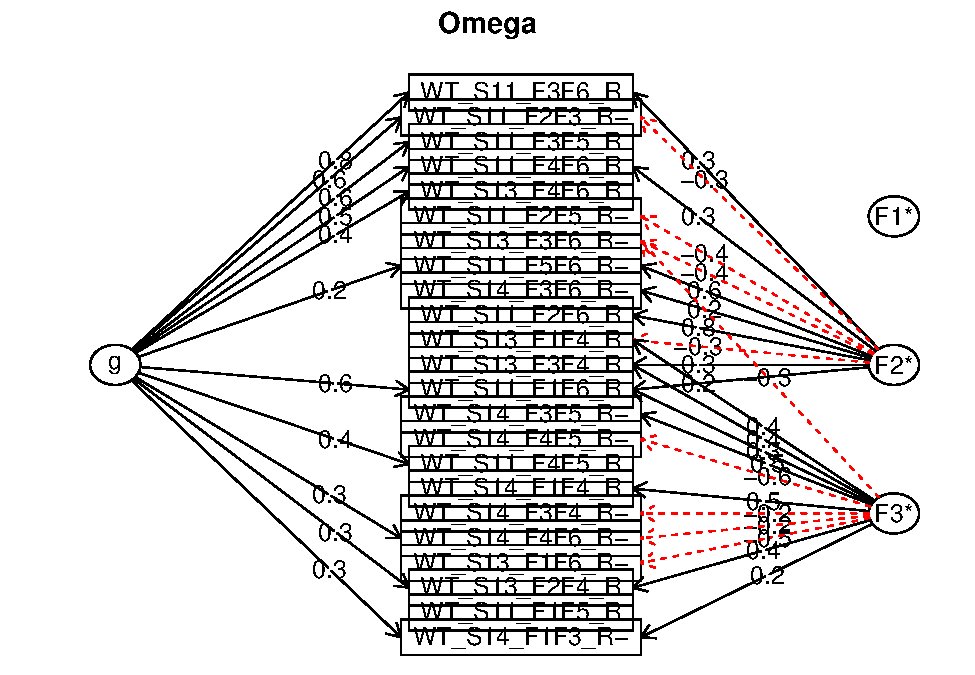
\includegraphics{expertise_2024_09_26_no_outlierdetection_MK_files/figure-latex/sjt_omega-3.pdf}
Omega Call: omegah(m = m, nfactors = nfactors, fm = fm, key = key, flip
= flip, digits = digits, title = title, sl = sl, labels = labels, plot =
plot, n.obs = n.obs, rotate = rotate, Phi = Phi, option = option, covar
= covar) Alpha: 0.65 G.6: 0.84 Omega Hierarchical: 0.69 Omega H
asymptotic: 0.94 Omega Total 0.74

Schmid Leiman Factor loadings greater than 0.2 g F1* F2* F3* h2 h2 u2 p2
com WT\_S11\_F1F5\_R 0.06 0.94 0.51 2.02 WT\_S11\_F1F6\_R 0.58 0.24 0.26
0.46 0.46 0.54 0.73 1.76 WT\_S11\_F2F3\_R- 0.62 -0.29 0.49 0.49 0.51
0.78 1.57 WT\_S11\_F2F5\_R- -0.38 0.16 0.84 0.11 1.26 WT\_S11\_F2F6\_R
0.80 0.68 0.68 0.32 0.04 1.12 WT\_S11\_F3F5\_R 0.60 0.37 0.37 0.63 0.96
1.09 WT\_S11\_F3F6\_R 0.79 0.33 0.73 0.73 0.27 0.84 1.36
WT\_S11\_F4F5\_R 0.41 0.22 0.22 0.78 0.76 1.64 WT\_S11\_F4F6\_R 0.51
0.27 0.36 0.36 0.64 0.72 1.80 WT\_S11\_F5F6\_R- 0.21 0.59 0.40 0.40 0.60
0.11 1.26 WT\_S13\_F1F4\_R -0.33 0.41 0.29 0.29 0.71 0.02 1.99
WT\_S13\_F1F6\_R- -0.50 0.29 0.29 0.71 0.11 1.28 WT\_S13\_F2F4\_R 0.26
0.38 0.21 0.21 0.79 0.33 1.81 WT\_S13\_F3F4\_R 0.25 0.37 0.21 0.21 0.79
0.07 2.01 WT\_S13\_F3F6\_R- -0.38 -0.33 0.26 0.26 0.74 0.05 2.17
WT\_S13\_F4F6\_R 0.40 0.19 0.81 0.85 1.35 WT\_S14\_F1F3\_R- 0.34 0.24
0.18 0.82 0.67 1.81 WT\_S14\_F1F4\_R 0.55 0.32 0.32 0.68 0.01 1.12
WT\_S14\_F3F4\_R- -0.22 0.07 0.93 0.22 2.00 WT\_S14\_F3F5\_R- 0.49 0.30
0.30 0.70 0.10 1.49 WT\_S14\_F3F6\_R- 0.24 0.07 0.93 0.19 1.48
WT\_S14\_F4F5\_R- -0.64 0.43 0.43 0.57 0.01 1.14 WT\_S14\_F4F6\_R- 0.26
-0.23 0.12 0.88 0.54 2.13

With Sums of squares of: g F1* F2* F3* h2 2.80 0.01 1.97 2.11 2.75

general/max 1.02 max/min = 211.46 mean percent general = 0.38 with sd =
0.34 and cv of 0.89 Explained Common Variance of the general factor =
0.41

The degrees of freedom are 187 and the fit is 6.03 The number of
observations was 72 with Chi Square = 365.08 with prob \textless{}
1.3e-13 The root mean square of the residuals is 0.1 The df corrected
root mean square of the residuals is 0.12 RMSEA index = 0.114 and the 10
\% confidence intervals are 0.098 0.133 BIC = -434.66

Compare this with the adequacy of just a general factor and no group
factors The degrees of freedom for just the general factor are 230 and
the fit is 8.49 The number of observations was 72 with Chi Square =
525.16 with prob \textless{} 4e-25 The root mean square of the residuals
is 0.15 The df corrected root mean square of the residuals is 0.16

RMSEA index = 0.133 and the 10 \% confidence intervals are 0.119 0.15
BIC = -458.47

Measures of factor score adequacy\\
g F1* F2* F3* Correlation of scores with factors 0.93 0.06 0.9 0.87
Multiple R square of scores with factors 0.86 0.00 0.8 0.76 Minimum
correlation of factor score estimates 0.72 -0.99 0.6 0.52

Total, General and Subset omega for each subset g F1* F2* F3* Omega
total for total scores and subscales 0.74 NA 0.67 0.44 Omega general for
total scores and subscales 0.69 NA 0.63 0.35 Omega group for total
scores and subscales 0.05 NA 0.04 0.09

\subsubsection{2.4 Classroom
Questionnaire}\label{classroom-questionnaire}

\begin{longtable}[]{@{}
  >{\raggedright\arraybackslash}p{(\columnwidth - 18\tabcolsep) * \real{0.0833}}
  >{\raggedleft\arraybackslash}p{(\columnwidth - 18\tabcolsep) * \real{0.0357}}
  >{\raggedleft\arraybackslash}p{(\columnwidth - 18\tabcolsep) * \real{0.0595}}
  >{\raggedleft\arraybackslash}p{(\columnwidth - 18\tabcolsep) * \real{0.0714}}
  >{\raggedleft\arraybackslash}p{(\columnwidth - 18\tabcolsep) * \real{0.0833}}
  >{\raggedleft\arraybackslash}p{(\columnwidth - 18\tabcolsep) * \real{0.0833}}
  >{\raggedleft\arraybackslash}p{(\columnwidth - 18\tabcolsep) * \real{0.1310}}
  >{\raggedleft\arraybackslash}p{(\columnwidth - 18\tabcolsep) * \real{0.1429}}
  >{\raggedleft\arraybackslash}p{(\columnwidth - 18\tabcolsep) * \real{0.1548}}
  >{\raggedleft\arraybackslash}p{(\columnwidth - 18\tabcolsep) * \real{0.1548}}@{}}
\caption{Mean, SD, min, max for classroom managament (cm) and
non-/paraverbal communication (n\&pv com)}\tabularnewline
\toprule\noalign{}
\begin{minipage}[b]{\linewidth}\raggedright
Group
\end{minipage} & \begin{minipage}[b]{\linewidth}\raggedleft
N
\end{minipage} & \begin{minipage}[b]{\linewidth}\raggedleft
M cm
\end{minipage} & \begin{minipage}[b]{\linewidth}\raggedleft
SD cm
\end{minipage} & \begin{minipage}[b]{\linewidth}\raggedleft
Min cm
\end{minipage} & \begin{minipage}[b]{\linewidth}\raggedleft
Max cm
\end{minipage} & \begin{minipage}[b]{\linewidth}\raggedleft
M n\&pv com
\end{minipage} & \begin{minipage}[b]{\linewidth}\raggedleft
SD n\&pv com
\end{minipage} & \begin{minipage}[b]{\linewidth}\raggedleft
Min n\&pv com
\end{minipage} & \begin{minipage}[b]{\linewidth}\raggedleft
Max n\&pv com
\end{minipage} \\
\midrule\noalign{}
\endfirsthead
\toprule\noalign{}
\begin{minipage}[b]{\linewidth}\raggedright
Group
\end{minipage} & \begin{minipage}[b]{\linewidth}\raggedleft
N
\end{minipage} & \begin{minipage}[b]{\linewidth}\raggedleft
M cm
\end{minipage} & \begin{minipage}[b]{\linewidth}\raggedleft
SD cm
\end{minipage} & \begin{minipage}[b]{\linewidth}\raggedleft
Min cm
\end{minipage} & \begin{minipage}[b]{\linewidth}\raggedleft
Max cm
\end{minipage} & \begin{minipage}[b]{\linewidth}\raggedleft
M n\&pv com
\end{minipage} & \begin{minipage}[b]{\linewidth}\raggedleft
SD n\&pv com
\end{minipage} & \begin{minipage}[b]{\linewidth}\raggedleft
Min n\&pv com
\end{minipage} & \begin{minipage}[b]{\linewidth}\raggedleft
Max n\&pv com
\end{minipage} \\
\midrule\noalign{}
\endhead
\bottomrule\noalign{}
\endlastfoot
Expert & 41 & 3.2 & 0.72 & 1 & 4 & 3.30 & 0.65 & 1 & 4 \\
Novice & 42 & 3.0 & 0.77 & 1 & 4 & 3.13 & 0.73 & 1 & 4 \\
\end{longtable}

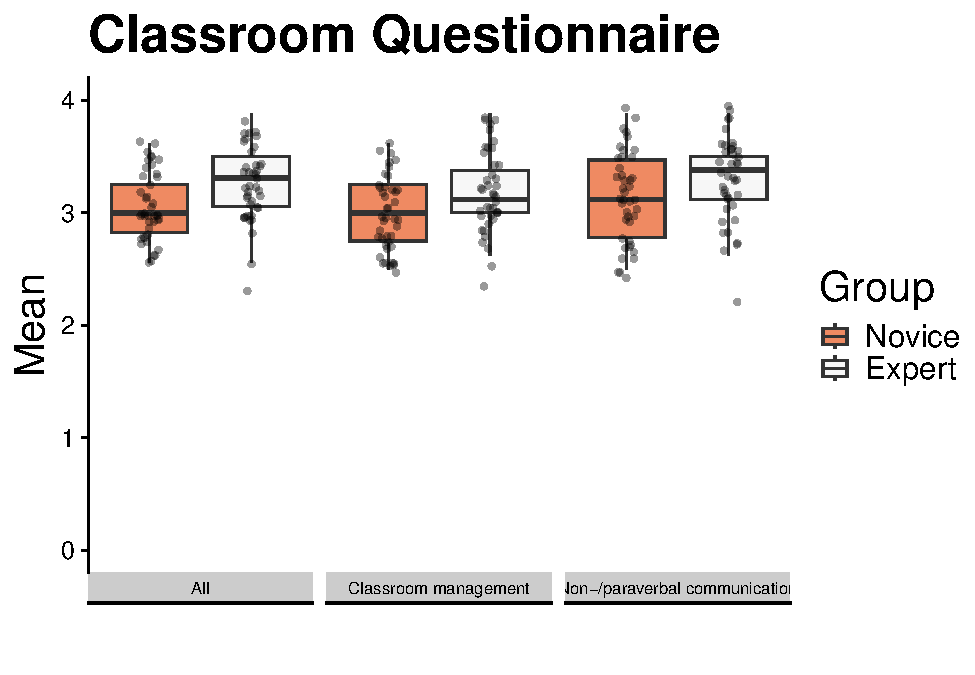
\includegraphics{expertise_2024_09_26_no_outlierdetection_MK_files/figure-latex/classroom questionnaire-1.pdf}

\paragraph{t-test \& effect size ``Classroom Questionnaire -
All''}\label{t-test-effect-size-classroom-questionnaire---all}

\begin{verbatim}
Two Sample t-test
\end{verbatim}

data: df\_quest\_plot\(All[df_quest_plot\)Group == ``Expert''{]} and
df\_quest\_plot\(All[df_quest_plot\)Group == ``Novice''{]} t = 2.7419,
df = 81, p-value = 0.007516 alternative hypothesis: true difference in
means is not equal to 0 95 percent confidence interval: 0.05014992
0.31545984 sample estimates: mean of x mean of y 3.247805 3.065000

{[}1{]} 0.6 attr(,``magnitude'') {[}1{]} ``medium''

\paragraph{t-test \& effect size ``Classroom Questionnaire - Classroom
Management''}\label{t-test-effect-size-classroom-questionnaire---classroom-management}

\begin{verbatim}
Two Sample t-test
\end{verbatim}

data: df\_quest\_plot\(`Classroom management`[df_quest_plot\)Group ==
``Expert''{]} and
df\_quest\_plot\(`Classroom management`[df_quest_plot\)Group ==
``Novice''{]} t = 2.6421, df = 81, p-value = 0.009887 alternative
hypothesis: true difference in means is not equal to 0 95 percent
confidence interval: 0.04912362 0.34875094 sample estimates: mean of x
mean of y 3.195366 2.996429

{[}1{]} 0.58 attr(,``magnitude'') {[}1{]} ``medium''

\paragraph{t-test \& effect size ``Classroom Questionnaire -
Non-/paraverbal
communication''}\label{t-test-effect-size-classroom-questionnaire---non-paraverbal-communication}

\begin{verbatim}
Two Sample t-test
\end{verbatim}

data:
df\_quest\_plot\(`Non-/paraverbal communication`[df_quest_plot\)Group ==
``Expert''{]} and
df\_quest\_plot\(`Non-/paraverbal communication`[df_quest_plot\)Group ==
``Novice''{]} t = 1.997, df = 81, p-value = 0.04919 alternative
hypothesis: true difference in means is not equal to 0 95 percent
confidence interval: 0.0006129687 0.3361233844 sample estimates: mean of
x mean of y 3.301463 3.133095

{[}1{]} 0.44 attr(,``magnitude'') {[}1{]} ``small''

\subsection{3. Correlations}\label{correlations}

\begin{verbatim}
## 
##  Pearson's product-moment correlation
## 
## data:  df_merge$GRI_mtu and df_merge$SJT_All
## t = -2.1712, df = 80, p-value = 0.03288
## alternative hypothesis: true correlation is not equal to 0
## 95 percent confidence interval:
##  -0.43084846 -0.01990909
## sample estimates:
##       cor 
## -0.235897
\end{verbatim}

\begin{verbatim}
## 
##  Pearson's product-moment correlation
## 
## data:  df_merge$GRI_mtu and df_merge$Quest_All
## t = 0.64655, df = 80, p-value = 0.5198
## alternative hypothesis: true correlation is not equal to 0
## 95 percent confidence interval:
##  -0.1472121  0.2846518
## sample estimates:
##        cor 
## 0.07209825
\end{verbatim}

\begin{verbatim}
## 
##  Pearson's product-moment correlation
## 
## data:  df_merge$GRI_mtu and df_merge$Mean_disruption_appraisal
## t = 0.60918, df = 80, p-value = 0.5441
## alternative hypothesis: true correlation is not equal to 0
## 95 percent confidence interval:
##  -0.1512868  0.2808174
## sample estimates:
##        cor 
## 0.06795118
\end{verbatim}

\begin{verbatim}
## 
##  Pearson's product-moment correlation
## 
## data:  df_merge$GRI_mtu and df_merge$Mean_confidence_appraisal
## t = -0.11168, df = 80, p-value = 0.9114
## alternative hypothesis: true correlation is not equal to 0
## 95 percent confidence interval:
##  -0.2288719  0.2050778
## sample estimates:
##        cor 
## -0.0124849
\end{verbatim}

\begin{verbatim}
## 
##  Pearson's product-moment correlation
## 
## data:  df_merge_experts$GRI_mtu and df_merge_experts$`Teaching Experience`
## t = -1.4152, df = 38, p-value = 0.1652
## alternative hypothesis: true correlation is not equal to 0
## 95 percent confidence interval:
##  -0.50038371  0.09433299
## sample estimates:
##        cor 
## -0.2237514
\end{verbatim}

\end{document}
